\documentclass[orivec]{llncs}
\usepackage{graphicx}
\usepackage{amsmath}		% for "cases"
\usepackage{amsfonts}		% for frakur fonts
\usepackage{mathrsfs}		% for curly "E" error symbol
\usepackage{float}
\usepackage{tcolorbox}		% for wrapping example in color box
\usepackage{wrapfig}		% wrap figure beside text, used in example
\usepackage{tikz-cd}		% commutative diagrams
% \usepackage{amsfonts}
\usepackage{amssymb}		% for \multimap, \updownarrow, \bigstar
\usepackage{sectsty}		% change section color

% *************** Delete when not using Chinese or colors **********************
\usepackage{xeCJK}
\setCJKmainfont[BoldFont=SimHei,ItalicFont=KaiTi]{SimSun}
\usepackage{color}
\newcommand{\emp}[1]{\textbf{\textcolor{blue}{#1}}}

\sectionfont{\color{blue}} 
\subsectionfont{\color{blue}} 
\subsubsectionfont{\color{blue}} 
\definecolor{green}{rgb}{0,0.7,0}

\usepackage{geometry}		% change paper size
\geometry{
  a4paper,         % or letterpaper
  textwidth=18cm,  % llncs has 12.2cm
  textheight=27cm, % llncs has 19.3cm
  heightrounded,   % integer number of lines
  hratio=1:1,      % horizontally centered
  vratio=2:3,      % not vertically centered
}
\usepackage[fontsize=13pt]{scrextend}

\newcommand{\vect}[1]{\boldsymbol{#1}}
\newcommand*\sigmoid{\vcenter{\hbox{
\includegraphics{sigmoid.png}}}}
\newcommand*\rectifier{\vcenter{\hbox{
\includegraphics{rectifier.png}}}}
\newcommand{\dashh}{\textemdash~}
\newcommand{\english}[1]{\rmfamily \textit{``#1''}\rmfamily}

% ***** Boxed variables inside math equations
% \newcommand*{\boxedcolor}{black}
\makeatletter
% \renewcommand{\boxed}[1]{\textcolor{\boxedcolor}{%
% \fbox{\normalcolor\m@th$\displaystyle#1$}}}
% \setlength{\fboxsep}{1pt}
\renewcommand{\boxed}[1]{\fbox{\m@th$\displaystyle\scalebox{0.9}{#1}$} \,}
\makeatother

\overfullrule=0mm

\newsavebox{\MyName}
\savebox{\MyName}{
\includegraphics[scale=0.6]{YKY.png}}

\title{Wandering in the Labyrinth of Thinking\\
\normalsize{-- a cognitive architecture combining reinforcement learning\\
and deep learning}}
\titlerunning{Wandering in the Maze of Thinking}
\author{\usebox{\MyName} (King-Yin Yan)
% \\ \footnotesize{General.Intelligence@Gmail.com}
\and
Ben Goertzel
\and
Juan Carlos Kuri Pinto
}
\institute{General.Intelligence@Gmail.com}

\begin{document}

\maketitle

\setlength{\parindent}{0em}
\setlength{\parskip}{2.8ex plus0.8ex minus0.8ex}
% \setlength{\parskip}{2.8ex}

\begin{abstract}
% 介绍一个基於 \textbf{增强学习} 和 \textbf{深度学习} 的极简约的 cognitive architecture,它在数学上是一个Hamiltonian 系统,而其 Lagrangian 对应於智能系统的「奖励」或「欲望」的价值。 经典逻辑 AI 的技巧可以搬到这个 setting 之下,而连续时间化之后,可以用上微分几何的技巧。 
Introducing a minimalist cognitive architecture based on DRL (deep reinforcement learning).  Mathematically it is a Hamiltonian system, whose Lagrangian corresponds to the value of ``desires'' or ``rewards'' in the intelligent system.  Techniques of classical logic-based AI can be transferred to this setting.  Its continuous limit can be described by differential geometry.  The old-fashioned logic-based knowledge representation with discrete propositions is abandoned in favor of a representation induced by deep neural learning.
% The problem of general intelligence can be described and solved in the logic-based AI paradigm, but the main obstacle is that learning is too slow.  The logic-based knowledge representation with discrete propositions is abandoned in favor of a neural-based ``amorphous'' representation induced from the top down, using a deep neural network (DNN).  The DNN acts iteratively on a state space (the ``mental state''), forming a dynamical system.  This system is in turn controlled by reinforcement learning, ``navigating'' the space of mental states as in a maze.
\end{abstract}

%本文介绍一些(非原创的)已知理论,然后指出一些新的研究方向。
The first part of this paper introduces some existing theory, and then speculates on new research directions.

\section{Main idea}

The \textbf{metaphor} here is that of reinforcement learning controlling an autonomous agent to navigate the maze of ``thoughts space'':
\begin{equation}
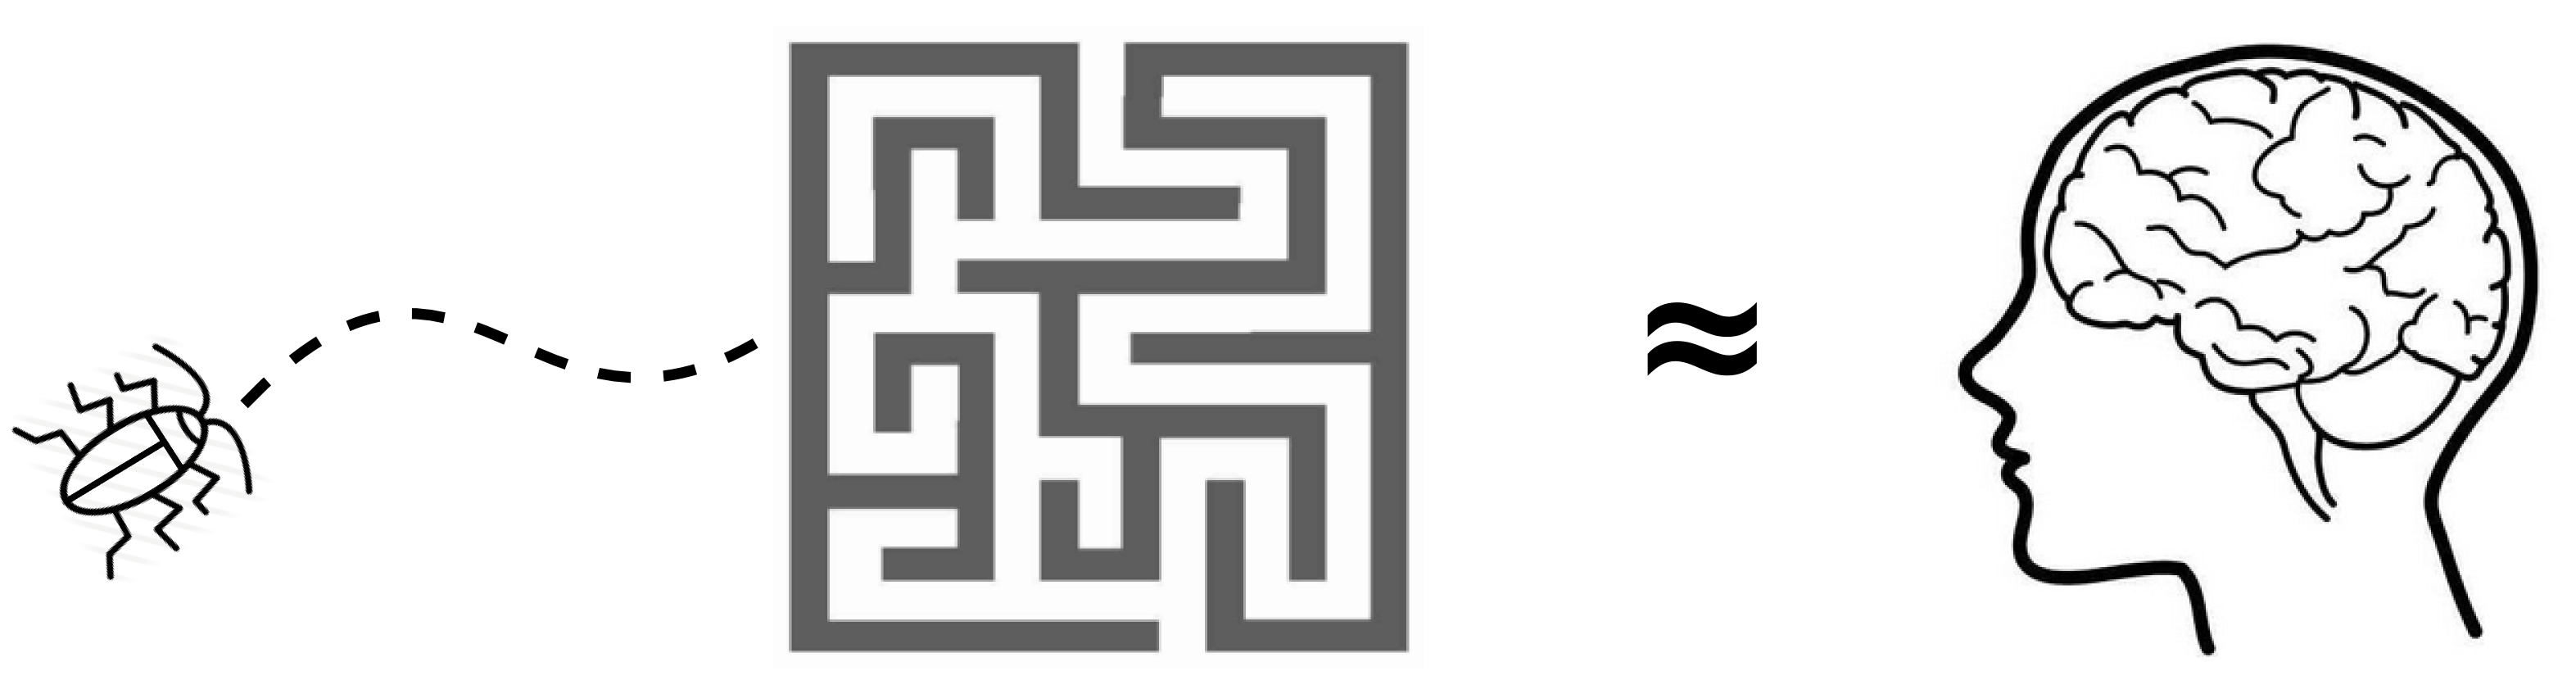
\includegraphics[scale=0.5]{maze-metaphor.png}
\end{equation}

The main idea is to regard ``thinking'' as a \emp{dynamical system} operating on \emp{mental states}:
\begin{equation}
\label{fig:mental-state}
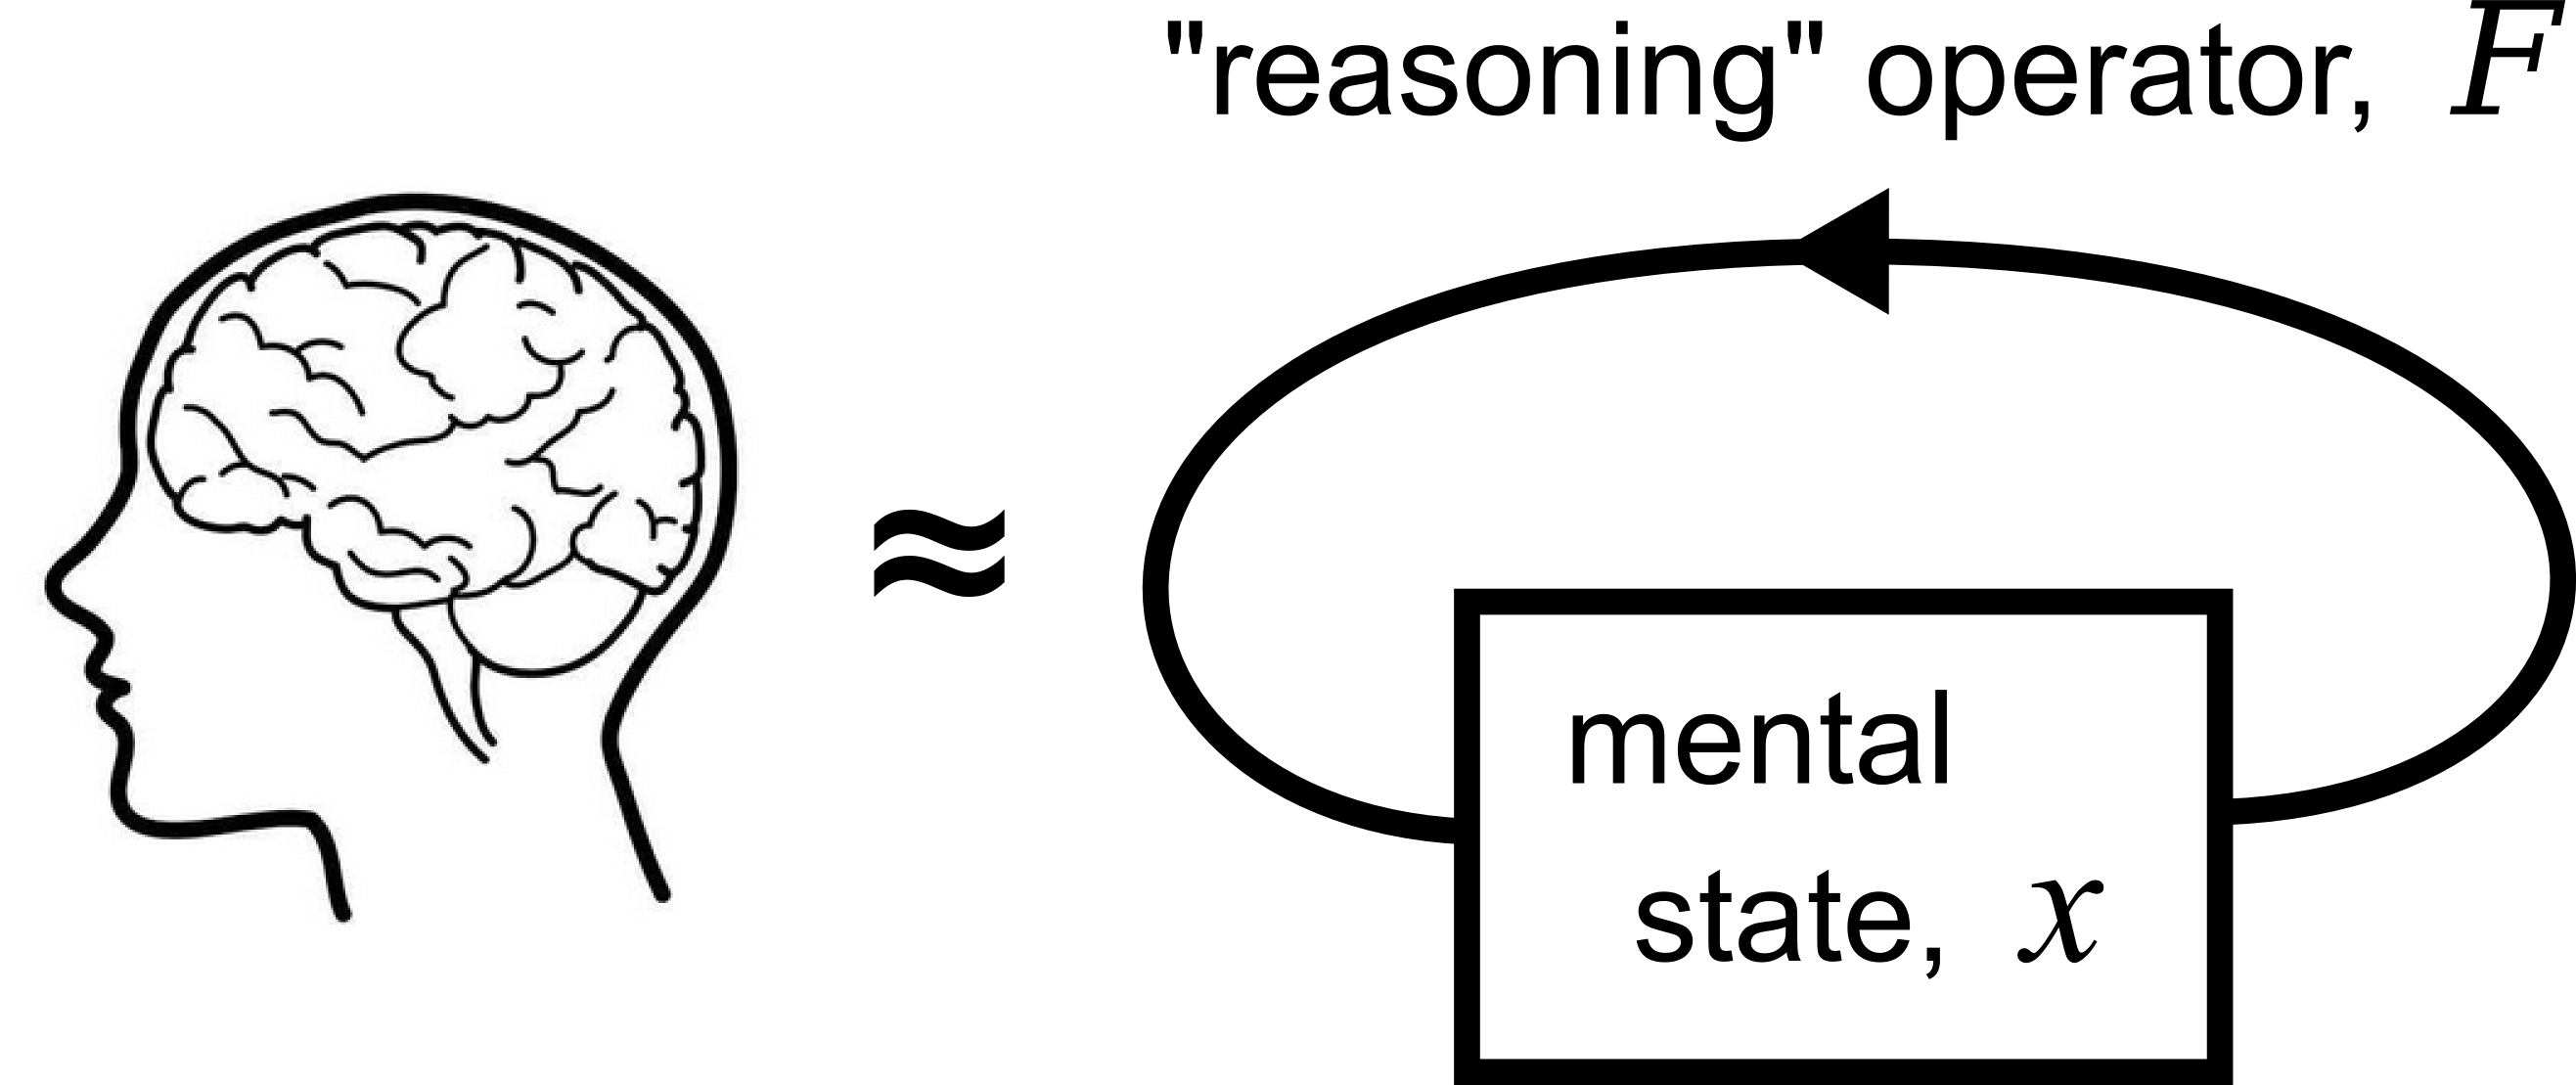
\includegraphics[scale=0.5]{mental-state.png}
\end{equation}

For example, a mental state could be the following set of propositions:
\let\labelitemi\labelitemii
\begin{itemize}
\item I am in my room, writing a paper for AGI-17.
\item I am in the midst of writing the sentence, ``I am in my room, ...''
\item I am about to write a gerund phrase ``writing a paper...''
\end{itemize}

Thinking is the process of \emp{transitioning} from one mental state to another.  Even as I am speaking now, I use my mental state to keep track of where I am at within the sentence's syntax, so that I can structure sentences grammatically.

By representing a cognitive state as a vector $\vec{x} \in X$ where $X$ is the cognitive state-space, the reasoning operator $R$ as an \emp{iterative map} $X \rightarrow X$, we would have at disposal all the tools available in vector space such as:

\begin{itemize}
\item numerical optimization (eg gradient descent)
\item differential equations governing time evolution
\item dynamical systems theory, control theory, dynamic programming, reinforcement learning
% \item Lie algebra and $C^*$-algebra of continuous operators
% \item matrix theory, iteration and fixed-point theory
\item neural networks and deep learning ... etc.
\end{itemize}

\subsection{Related work}

Google's \textbf{PageRank} is one of the earlier successful applications of vector-space and matrix techniques.  The \textbf{Word2Vec} \cite{Weston2015} algorithm that maps natural-language words to vectors is also spectacularly successful and influential;  it demonstrated the potential advantages of vector representations.  As for reinforcement learning, Q-learning (a form of RL) has been combined with deep learning to successfully play Atari games \cite{Mnih2013};  Their architecture is exactly the same as ours, except that we are trying to refine the internal structure of the learner.
%, both exploit the efficiency of vector and matrix calculus.

This is the cartoon version of our architecture:
\begin{equation}
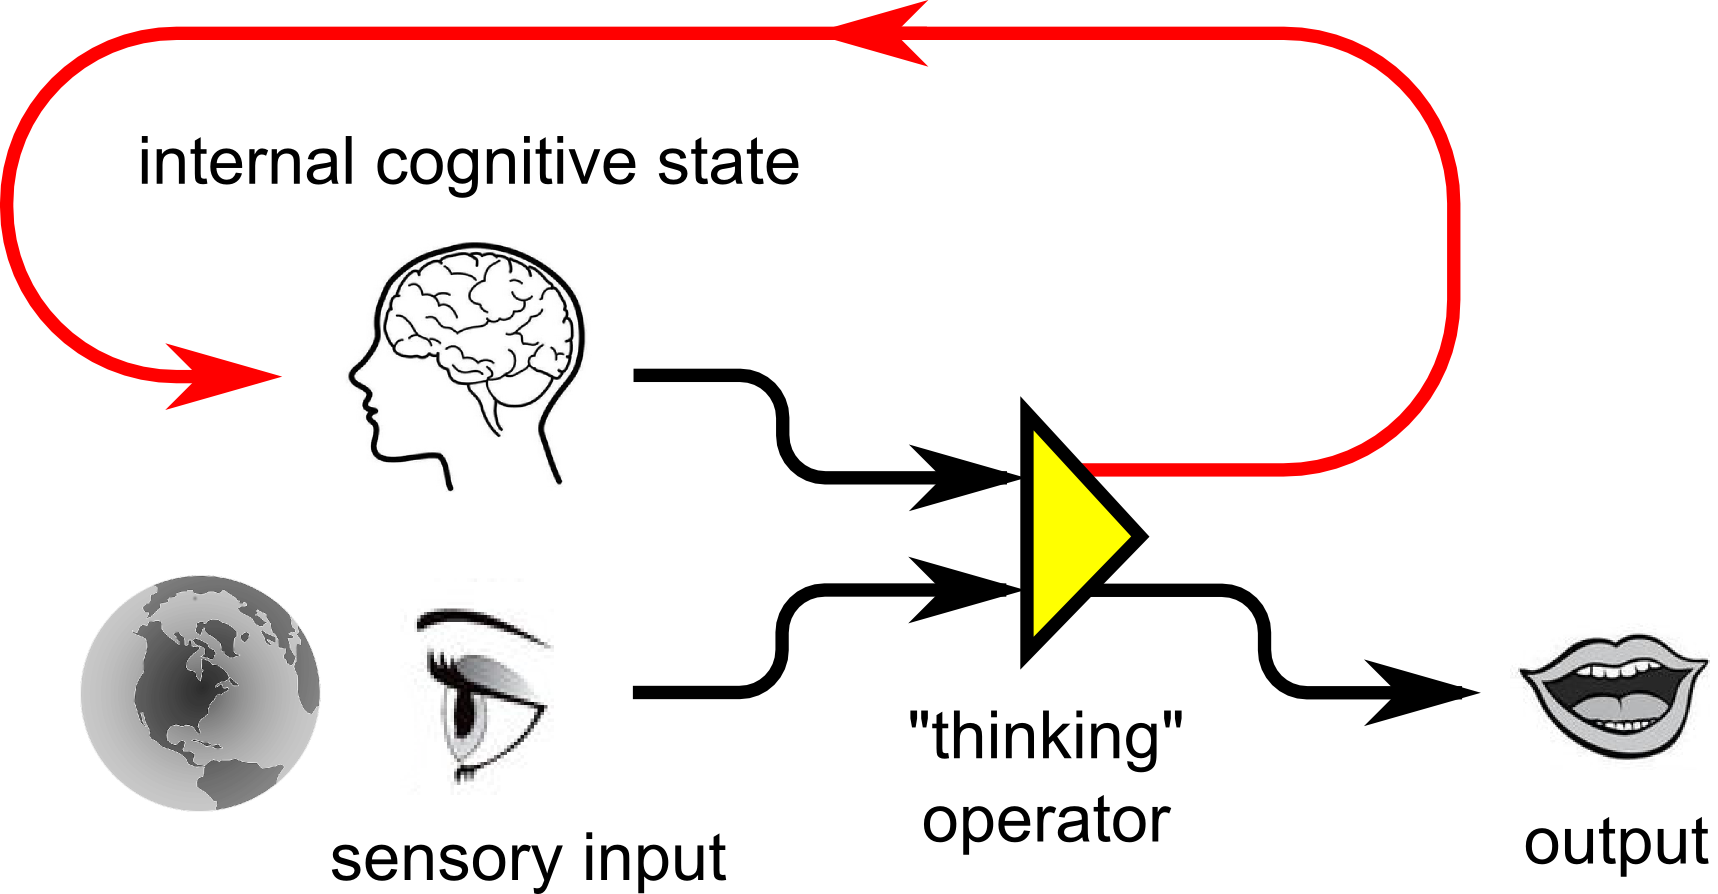
\includegraphics[scale=0.5]{architecture-cartoon.png}
\end{equation}

\section{Logic-based AI (LBAI)}

Main points:
\begin{itemize}
\item We would not directly implment logic-based AI, but it serves as a \textit{backdrop} for understanding what are the problems of general AI.
\item In this paper we would jump back and forth between the logic-based view and the dynamical state-space view.  Knowledge of LBAI is essential to understanding ideas in this paper.
\end{itemize}

% Having worked on LBAI for many years, I tend to look back to LBAI to understand a problem when designing an AI system.   因此我的思路喜欢将新问题还原到逻辑 AI 那边去理解,但实际上我提倡的解决办法不是靠经典逻辑,甚至不是 symbolic 的。  但在这篇文章我还是会经常跳回到逻辑 AI 去方便理解。

It is feasible to use mathematical logic to emulate human thinking, an approach pioneered by John McCarthy (1927-2011).  We have 3 basic operations: deduction, abduction, induction;  For details one can refer to 《Computational logic and human thinking》by Robert Kowalski, 2011. We would not waste time to debate whether LBAI is an adequate model of human thinking;  This paper assumes it as the point of departure.  It is worth mentioning though, that Kowalski is one of the researchers who laid the theoretical foundations of logic programming, especially Prolog.

In classical logic-based AI, ``thinking'' is achieved by steps like this:
\begin{eqnarray}
\mbox{premise} & \vdash & \mbox{conclusion} \\
\boxed{\mbox{it was raining this morning}} & \vdash & \boxed{\mbox{grass is wet}}
\end{eqnarray}
That is to say: from some \emp{propositions} we deduce other propositions.

Deduction requires some special propositions known as \emp{rules}, these are propositions containing \emp{variables} such as ``$x$'':
\begin{equation}
\boxed{\mbox{it is raining at location $x$}} \wedge \boxed{\mbox{$x$ is uncovered}} \vdash \boxed{\mbox{location $x$ is wet}}
\end{equation}
Rules are like the ``fuel'' for an inference engine;  The engine cannot run without fuel.

Note: The $x$ inside a proposition is like a ``hole'' in it.  We could use \emp{substitution} to place some concrete \emp{objects} into such holes, to make the proposition \textit{complete}.  This is a form of \emp{sub-propositional} structure, and one way to express it is via \emp{predicate logic}.  We don't need to concern with details right now.

LBAI can be viewed as the compression of a world model into a knowledge-base (KB) of logic formulas (that consists of \textbf{facts} as well as \textbf{rules}):
\begin{equation}
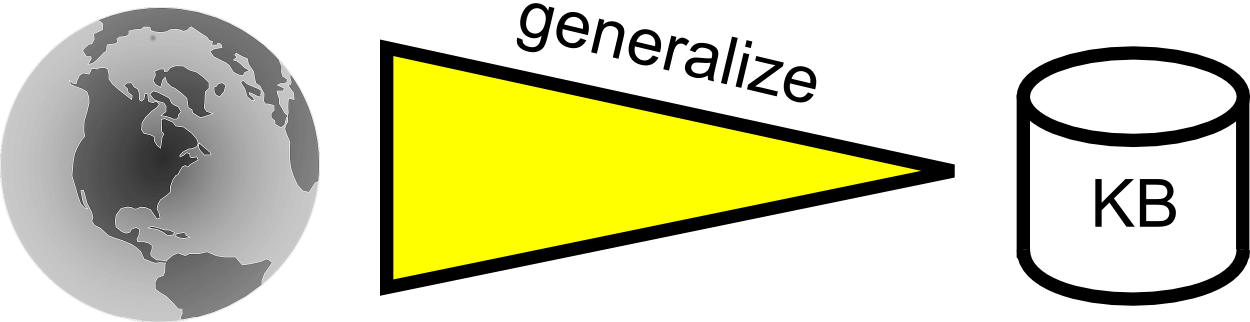
\includegraphics[scale=0.5]{world-model-compression.png}
\end{equation}
The world model is \textit{generated} combinatorially from the set of logic formulas, vaguely reminiscent of a ``basis'' in vector space.  The generative process in logic is much more complicated, contributing to its high \textit{compressive} ability on the one hand, and the \textit{complexity} of learning such formulas on the other hand.

\subsection{Bottom-up vs top-down representations}

In LBAI the knowledge representation structure is built (\textit{fixed}) from the bottom up (For example, predicate symbols and constant symbols build up propositions, and sets of propositions form theories):
%\begin{equation}
%\mbox{words } \triangleright \mbox{ sentences } \triangleright \mbox{ logical form } \triangleright \mbox{ logical KB}
%\end{equation}
%Thus the structure of the KB is \textit{fixed} by the human designer. % This rigidity is perhaps why learning in logic-based systems is slow.

% In natural language, an idea can be expressed as a concatenation of words, for example:\\
% And it is just a short jump from word concatenations to symbolic logic.  But this jump may land us into a logic-based ``tar pit'', in which everything is theoretically possible, but often too slow in practice.

%It is just a short jump from the expression of ideas as word concatenations to logical form as linear (or tree-like, or graph-like) compositions of symbols:
\begin{equation}
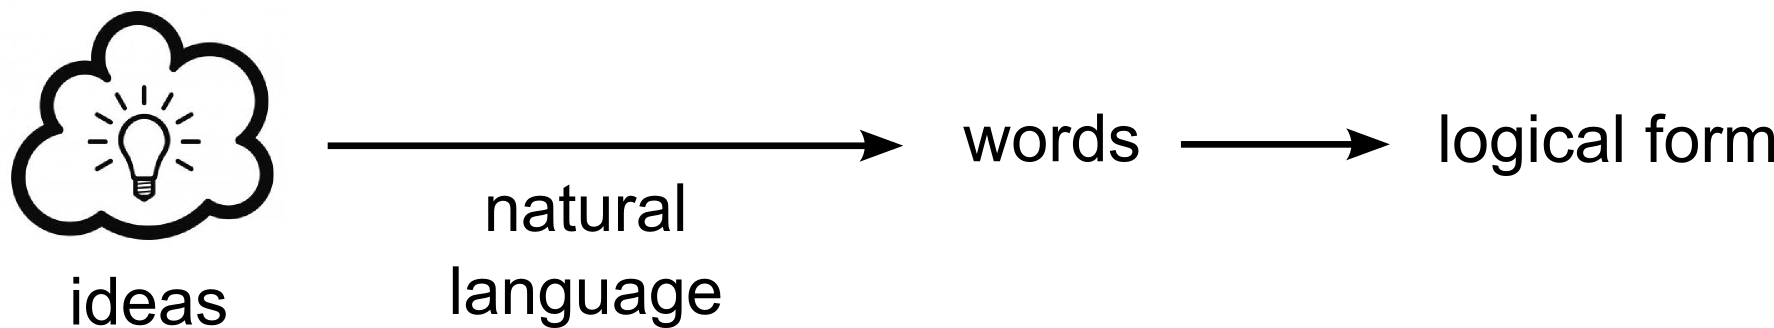
\includegraphics[scale=0.5]{ideas-vs-logical-form.png}
\end{equation}
but is it valid (or profitable) to assume that our mental representations are \textit{isomorphic} to such logical structures?  Or drastically different?

The most serious disadvantage of bottom-up representations lies in the difference between \emp{syntactic distance} and \emp{semantic distance}.  Suppose propositions are built up from an ``alphabet'' of atomic concepts, through the use of a multiplication operation such as tensor product.  We embed atomic concepts into a vector space, in the manner of the Word2Vec algorithm.  Then, using the tensor product, propositions (ie sentences) will be mapped to positions in the tensor-product vector space.  Thus we can measure the \textbf{distance} between any two propositions.  However, this is a \textbf{syntactic} distance.  For example, \textit{``Don't judge a book by its cover''} and \textit{``Clothes do not make the man''} are superficially very different (syntactically distant) but are semantically close.  In a good learning system we need to \textbf{generalize} according to semantic distance.  The embedding of bottom-up representations usually gives us a discrete space with fractal structure, and the metric defined on such a space is always syntactic.

Humans are good at designing symbolic structures, but we don't know how to design \textit{neural} representations which are more or less opaque to us.
Perhaps we could use a neural network acting recurrently on the state vector to \emp{induce} an internal representation of mental space.  ``\textit{Induced by what},'' you ask?  By the very structure of the neural network itself.  In other words, forcing a neural network to \textit{approximate} the ideal operator $R^*$.

From an abstract point of view, we require:
\begin{itemize}
\item $R$ be an endomorphism: $X \rightarrow X$
\item $R$ has a learning algorithm: $R \stackrel{A}{\longmapsto} R^*$
\end{itemize}

$R$ would contain all the knowledge of the KB, so we expect it to be ``large'' (eg. having a huge number of parameters).  We also desire $R$ to possess a \emp{hierarchical} structure because hierarchies are computationally very efficient.  A multi-layer perceptron (MLP) seems to be a good candidate, as it is just a bunch of numbers (weight matrices $W$) interleaved by non-linear activation functions:
\begin{equation}
R(\vect{x}) = \sigmoid(W_1 \sigmoid(W_2 ... \sigmoid(W_L \vect{x} )))
\end{equation}
where $L$ is the number of layers.  MLPs would be our starting point to explore more design options.

In 1991 Siegelmann and Sontag \cite{Siegelmann1991} proved that recurrent neural networks (RNNs) can emulate any Turing machine.  In 1993 James Lo \cite{Lo1993} proved that RNNs can universally approximate any non-linear dynamical system.

The idea of $R$ as an operator acting on the state is inspired by the ``consequence operator'' in logic, usually denoted as $\mbox{Cn}$:
\begin{equation}
\mbox{Cn}(\Gamma) = \{ \mbox{ set of propositions that entails from } \Gamma \; \}
\end{equation}
but the function of $R$ can be broader than logical entailment.  We could use $R$ to perform the following functions which are central to LBAI:
\begin{itemize}
\item \emp{deduction} -- forward- and backward-chaining
\item \emp{abduction} -- finding explanations
\item \emp{inductive learning}
\end{itemize}

Below, we try to formalize the structure of logic from 2 perspectives:
\begin{itemize}
\item Static structure (formulas built from atomic concepts, logic operators, etc)
\item Dynamic structure (mechanisms of proof, inference, etc)
\end{itemize}

\subsection{Static structure of logic}

\begin{itemize}
\item \emp{truth values} (eg. P(rain tomorrow) = 0.7)
\item \emp{propositional structure} (eg. conjunction: $A \wedge B$) 
\item \emp{sub-propositional structure} (eg. predication: loves(john, mary) )
\item \emp{subsumption structure} (eg. $\mbox{dog} \subseteq \mbox{animal}$)
\end{itemize}

These structures can be ``transplanted'' to the vector space $X$ via:
\begin{itemize}
\item \emp{truth values: } an extra dimension conveying the ``strength'' of states
\item \emp{propositional structure: } eg. conjunction as vector addition,
\begin{equation}
A \wedge B \quad \Leftrightarrow \quad \vect{x}_A + \vect{x}_B + ...
\end{equation}
but we may have to avoid linear dependencies (``clashing'') such as:
\begin{equation}
\vect{x}_3 = a_1 \vect{x}_1 + a_2 \vect{x}_2
\end{equation}
This would force the vector space dimension to become very high.
\item \emp{sub-propositional structure: } eg. tensor products as composition of concept atoms:
\begin{equation}
\mbox{loves(john, pete)} \quad \Leftrightarrow \quad \overrightarrow{john} \otimes \overrightarrow{love} \otimes \overrightarrow{pete}
\end{equation}
\item \emp{subsumption structure: } eg. define the \textbf{positive cone} $C$ such that
\begin{equation}
\mbox{animal} \supseteq \mbox{dog} \quad \Leftrightarrow \quad \overrightarrow{animal} - \overrightarrow{dog} \in C
\end{equation}
\end{itemize}

But the more logical structure we add to $X$, the more it will resemble logic, and this whole exercise becomes pointless.  Remember our original goal is to try something different from logic, by \textit{relaxing} what defines a logical structure.  So we would selectively add features to $X$.

\subsection{Dynamic structure of logic}

{\color{green}@Andrew: This is where I want to formalize a ``logical system''.  Particularly, the state $X$ has internal structure that I have ignored so far:  $X$ should be a \textbf{set} of propositions.  During deduction, we need to \textbf{select} a few propositions from $X$ and try to \textbf{match} them with existing logic rules (this is the job of the famous \textbf{unifcation} algorithm in logical AI systems).  The selection is part of the control variable $u$ (see below).  We need to decompose the vector $X$ into some analogue of ``propositions'', but I don't know how to do it yet.  Perhaps elucidating the algebraic form of the logic system will help us design the ``vectorization'' scheme.
}

The 2 ``pillar'' algorithms for deduction in LBAI are:

\begin{itemize}
\item \emp{Resolution}:  deducing new propositions (conclusions) from existing ones (premises) \\
\begin{equation}
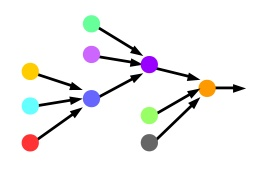
\includegraphics[scale=0.5]{resolution-cartoon.jpg}
\end{equation}
\item \emp{Unificaiton}:  matching a proposition with variables (``holes'') with grounded (``without holes'') propositions \\
\begin{equation}
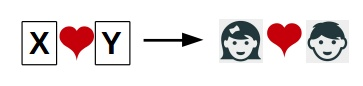
\includegraphics[scale=0.5]{unification-cartoon.jpg}
\end{equation}
\end{itemize}

The algebraization of first-order predicate logic (a logic whose propositions can have internal variables) is a difficult subject, potentially involving Tarski's cylindrical algebra which the author is unfamiliar with.

Here we introduce a crucial idea: using an \textbf{external memory} to manage the problem of \textbf{variable binding}.  Recall that a \textbf{Turing machine} is just a finite state machine equipped with a \textbf{memory tape};  It could be said that the memory tape is what enables the machine to have Turing-complete computing power.  Similarly, allowing a \textbf{propositional logic} to use an external memory storage for intermediate results, enables it to have the same expressive power as \textbf{predicate logic}.

Below are 2 cartoons illustrating how \textbf{resolution} and \textbf{unification} are performed with the aid of \textbf{external memory}:

{\color{green}@Andrew: I want to formalize these operations.  It may be more important than formalizing the \textbf{static} properties of logic.}

\begin{equation}
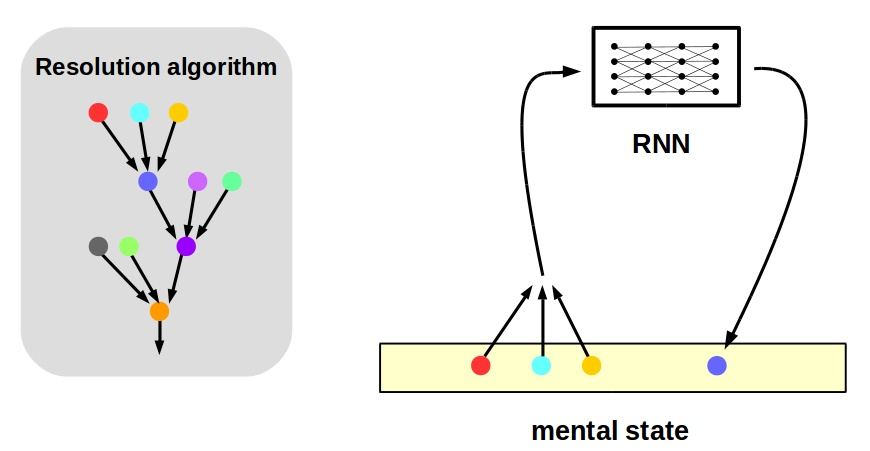
\includegraphics[scale=0.3]{resolution-cartoon-2.jpg}
\end{equation}

\begin{equation}
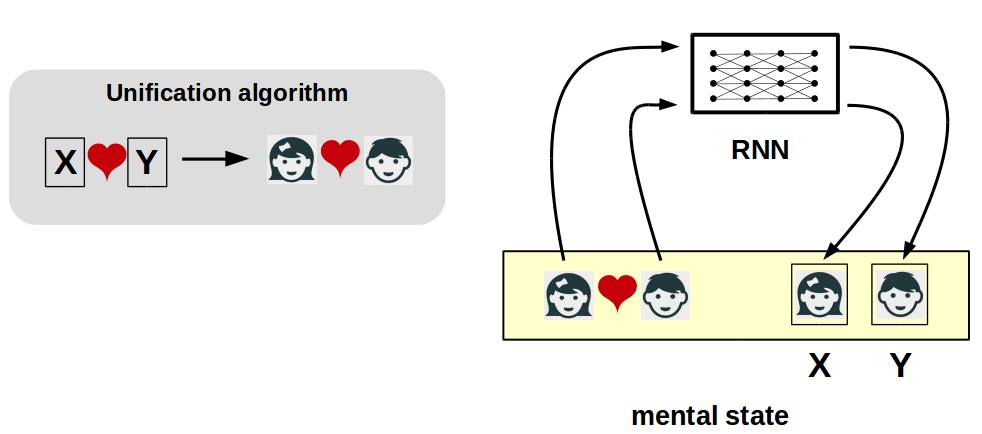
\includegraphics[scale=0.3]{unification-cartoon-2.jpg}
\end{equation}

%%%%%%%%%%%%%%%%%%%%%%%%%%%%%%% Example 1 %%%%%%%%%%%%%%%%%%%%%%%%%%%%%%%
\begin{tcolorbox}[width=\textwidth,colback={white},title={\centering \emp{Example 1: } primary-school arithmetic},colbacktitle=white,coltitle=black]

A recurrent neural network is a \textit{much more powerful} learning machine than a feed-forward network, even if they look the same superficially.

\begin{wrapfigure}{l}{2cm}
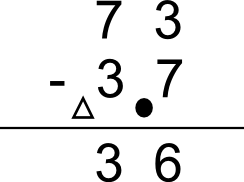
\includegraphics[scale=0.6]{elementary-arithmetic.png}
\end{wrapfigure} 

As an example, consider the way we perform 2-digit subtraction in primary school.  This is done in two steps, and we put a dot on paper to mark ``carry-over''.

The use of the paper is analogous to the ``tape'' in a Turing machine -- the ability to use short-term memory allows us to perform much more complex mental tasks.

We did a simple experiment to train a neural network to perform primary-school subtraction.  The operator is learned easily if we train the two steps \textit{separately}.  The challenge is to find an algorithm that can learn \emp{multi-step} operations by itself.

\end{tcolorbox}
%%%%%%%%%%%%%%%%%%%%%%%%%%%%%%%%%%%%%%%%%%%%%%%%%%%%%%%%%%%%%%%%%%%%%%%%%%

%%%%%%%%%%%%%%%%%%%%%%%%%%%%%%%% Example 2 %%%%%%%%%%%%%%%%%%%%%%%%%%%%%%%
\begin{tcolorbox}[width=\textwidth,colback={white},title={\centering \emp{Example 2: } variable binding in predicate logic},colbacktitle=white,coltitle=black]

The following formula in predicate logic defines the ``grandfather'' relation:

\begin{equation}
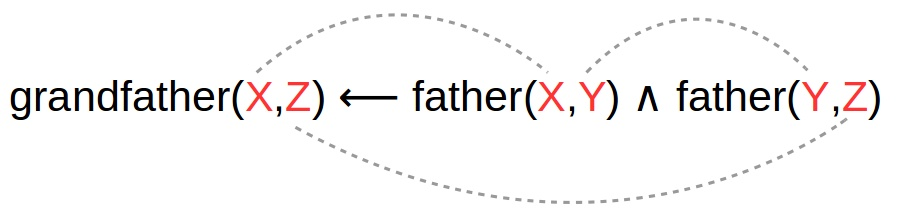
\includegraphics[scale=0.25]{linkage-in-logic-variables.jpg}
\end{equation}

We did a simple experiment to train a neural network to perform primary-school subtraction.  The operator is learned easily if we train the two steps \textit{separately}.  The challenge is to find an algorithm that can learn \emp{multi-step} operations by itself.

\end{tcolorbox}  
%%%%%%%%%%%%%%%%%%%%%%%%%%%%%%%%%%%%%%%%%%%%%%%%%%%%%%%%%%%%%%%%%%%%%%%%%%

\section{Control theory / reinforcement learning}

{\color{green}@Andrew: as you will see, the control theory part is essentially separated from the ``logic'' aspects.}

Main points:
\begin{itemize}
\item Intelligence is decomposed into \textbf{thinking} and \textbf{learning}.
\item \textbf{Thinking} is governed by control theory (finding the best trajectory in ``thoughts space'') under the contraints of correct reasoning, ie, knowledge.
\item The iterative ``thinking operator'' is implemented as a deep-\textbf{learning} neural network (DNN).  This DNN \textit{contrains} the dynamics of thinking, and it represents the totality of \textit{knowledge} in the system.
\end{itemize}

\begin{equation}
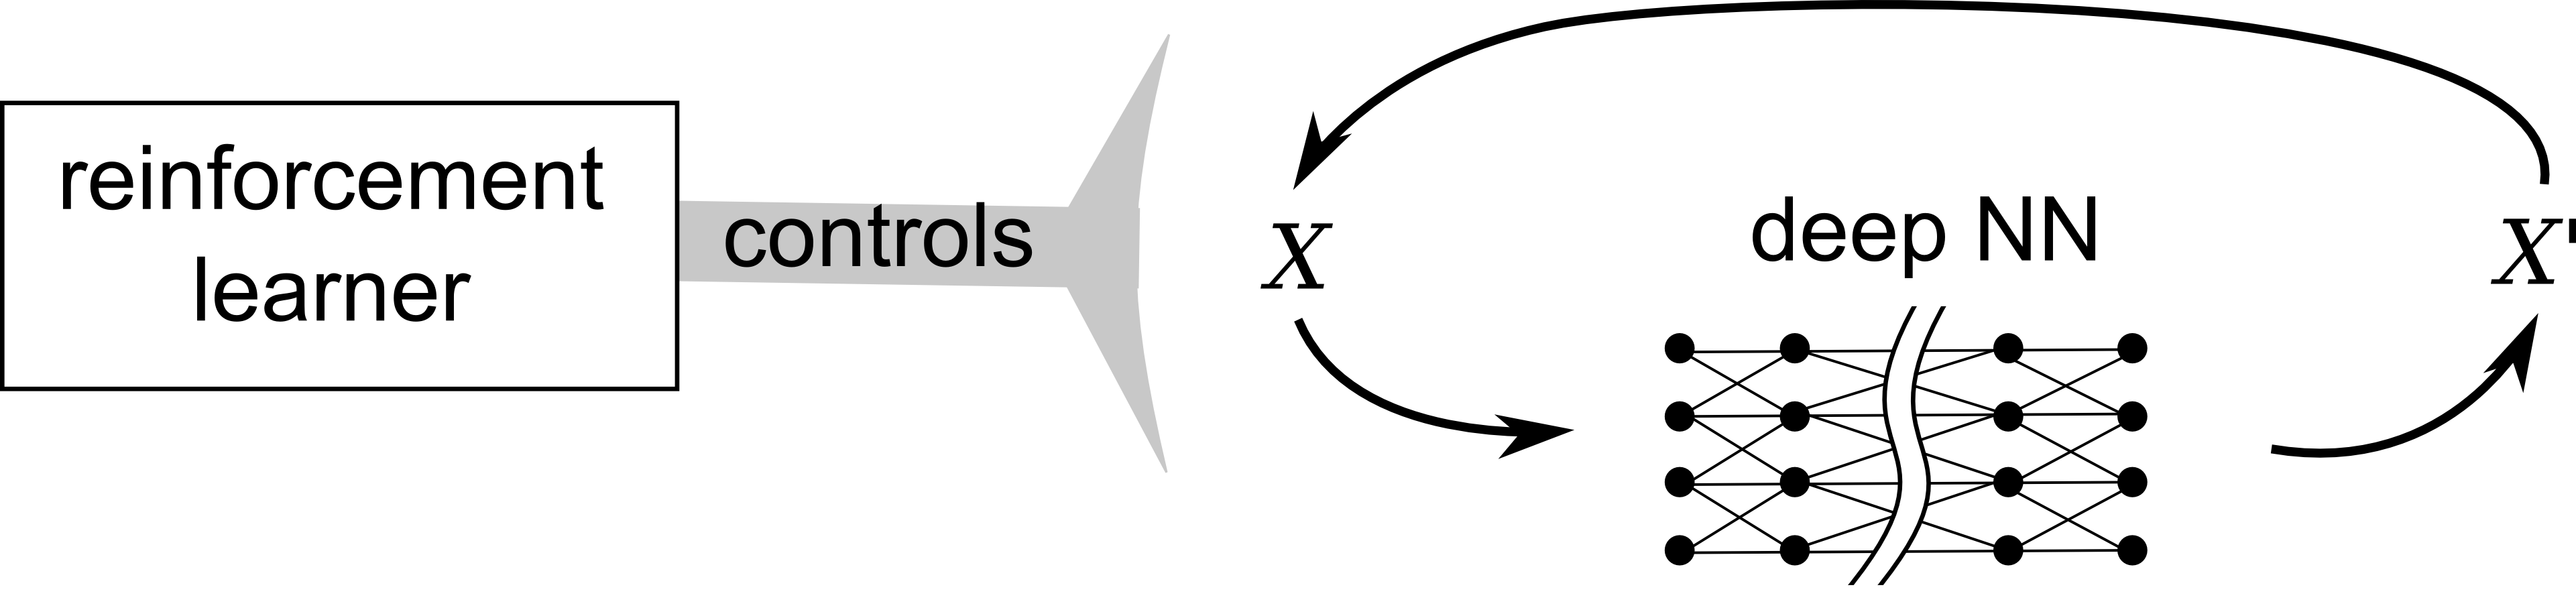
\includegraphics[scale=0.5]{genifer-model-0.png}
\end{equation}

\subsection{What is control theory?}

A \emp{dynamical system} can be defined by:
\begin{eqnarray}
\mbox{discrete time:} \quad \quad & \vect{x}_{t+1} = \vect{F}(\vect{x}_t) \\
\mbox{continuous time:} \quad \quad & \dot{\vect{x}} = \vect{f}(\vect{x}) \label{eqn1}
\end{eqnarray}
($\vect{F}$ is implemented as the deep learning network in our approach.)

A \emp{control system} can be defined as (sometimes I mix with continuous-time notation for the sake of simplicity):
\begin{equation}
\dot{\vect{x}}(t) = f(\vect{x}(t), \vect{u}(t), t)
\end{equation}
where $\vect{u}(t)$ is the \emp{control vector}.  The goal of control theory is to find the optimal $\vect{u}^*(t)$ function, such that the system moves from the initial state $\vect{x}_0$ to the terminal state $\vect{x_\bot}$.

\subsection{What is reinforcement learning?}

\textbf{Reinforcement learning} is synonymous with \textbf{dynamic programming}, which is also the main content of modern \textbf{control theory} with the state-space description.

The goal of \textbf{reinforcement learning} is to learn the \emp{policy function}:
\begin{equation}
\begin{tikzcd}[]
\mbox{policy : ~~state} \arrow[r, mapsto, "\scalebox{0.8}{action}"] & \mbox{state'}
\end{tikzcd}
\end{equation}
when we are given the \emp{state space}, \emp{action space}, and \emp{reward function}:
\begin{equation}
\mbox{reward}: \boxed{\mbox{state}} \times \boxed{\mbox{action}} \rightarrow \mathbb{R}
\end{equation}
The action $a$ is the same notion as the control variable $u$ in control theory.

The \emp{Bellman equation} governs reinforcement learning just as in control theory:
\begin{eqnarray}
\boxed{\mbox{optimal path}} = & \mbox{choose max reward on current path segment} \nonumber \\
& \quad + \boxed{\mbox{the rest of optimal path}}
\end{eqnarray}
In math notation:
\begin{equation}
U^*_t = \max_{u} \{ \; \boxed{\mbox{reward}(u, t)} + U^*_{t-1} \; \}
\end{equation}
where $U$ is the ``long-term value'' or \emp{utility} of a path.

Conceptually, $U$ is the \textbf{integration} of instantaneous rewards over time:
\begin{equation}
\boxed{\mbox{utility, or value} U} = \int \boxed{\mbox{reward} R} \,dt
\end{equation}

\subsection{Connection with Hamiltonian mechanics}

An interesting insight from control theory is that our system is a Hamiltonian dynamical system in a broad sense.

Hamilton's \emp{principle of least action} says that the trajectories of dynamical systems occuring in nature always choose to have their action $S$ taking \textbf{stationary values} when compared to neighboring paths.  The action is the time integral of the Lagrangian $L$:
\begin{equation}
\boxed{\mbox{Action} S} = \int \boxed{\mbox{Lagrangian} L} \; dt
\end{equation}
From this we see that the Lagrangian corresponds to the instantaneous ``rewards'' of our system.  It is perhaps not a coincidence that the Lagrangian has units of \textbf{energy}, in accordance with the folk psychology notion of ``positive energy'' when we talk about desirable things.

The \emp{Hamiltonian} $H$ arises when we consider a typical control theory problem;  The system is defined via:
\begin{eqnarray}
\mbox{state equation:} \quad & \dot{\vect{x}}(t) = \vect{f}[\vect{x}(t), \vect{u}(t), t] \\
\mbox{boundary condition:} \quad & \vect{x}(t_0) = \vect{x}_0 \,,\, \vect{x}(t_\bot) = \vect{x}_\bot \\
\mbox{objective function:} \quad & J = \int_{t_0}^{t_\bot} L[\vect{x}(t), \vect{u}(t), t] dt
\end{eqnarray}
The goal is to find the optimal control $\vect{u}^*(t)$.

Now apply the technique of \emp{Lagrange multipliers} for finding the maximum of a function, this leads to the new objective function:
\begin{equation}
U = \int_{t_0}^{t_\bot} \{ L + \vect{\lambda}^T(t) \left[ f(\vect{x}, \vect{u}, t) - \dot{\vect{x}} \right] \} dt
\end{equation}
So we can introduce a new scalar function $H$, ie the Hamiltonian:
\begin{equation}
H(\vect{x}, \vect{u}, t) = L(\vect{x}, \vect{u}, t) + \vect{\lambda}^T(t) f(\vect{x}, \vect{u}, t)
\end{equation}
Physically, the unit of $\vect{f}$ is velocity, while the unit of $L$ is energy, therefore $\vect{\lambda}$ should have the unit of \emp{momentum}.  This is the reason why the phase space is made up of the diad of $(\mbox{position}, \mbox{momentum})$.

In its most general form we have the \emp{Hamilton-Jacobi-Bellman equation}: \footnote{To digress a bit, this equation is also analogous to the \emp{Schr\"{o}dinger equation} in quantum mechanics:
\begin{equation}
i \hbar \frac{\partial}{\partial t} \Psi(x,t) = \left[ V(x,t) + \frac{-\hbar^2}{2\mu} \nabla^2 \right] \Psi(x,t).
\end{equation}
where $\Psi$ is analogous to our $U$ (perhaps $\Psi$ is something that nature wants to optimize?)}
\begin{equation}
\boxed{\mbox{Hamilton-Jacobi-Bellman}} \quad
0 = \frac{\partial U^*}{\partial t} + \min_u H
\end{equation}

All these ``physical'' ideas flow automatically from our definition of \textbf{rewards}, without the need to introduce them artificially.  But these ideas seem not immediately useful to our project, unless we are to explore \textbf{continuous-time} models.

\subsection{Deep learning}

The combination of deep learning with reinforcement learning, ie deep reinforcement learning (DRL), is very powerful.  For example, DRL is able to play Atari games to human levels \cite{Mnih2013}.  Their architecture is depicted in this diagram:
\begin{equation}
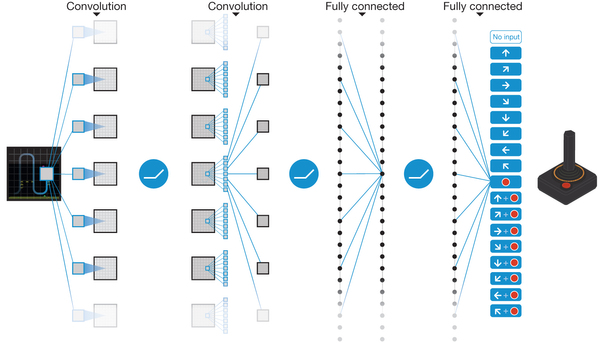
\includegraphics[scale=0.5]{Atari-Q-learning.jpg}
\end{equation}

Recall our main architecture:
\begin{equation}
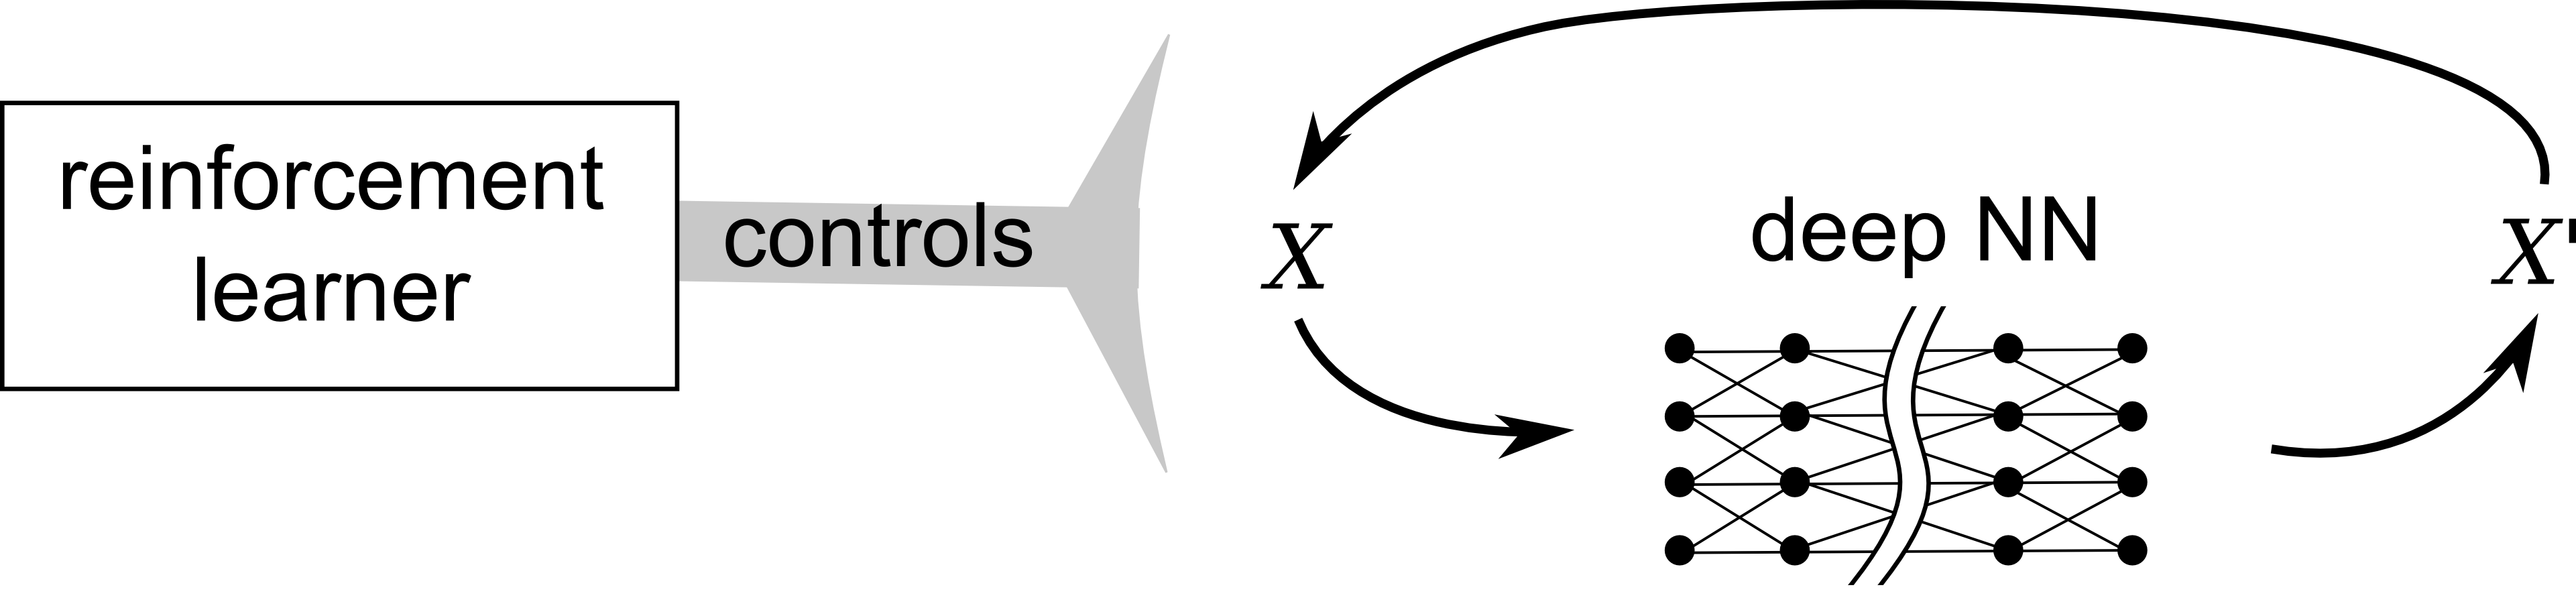
\includegraphics[scale=0.5]{genifer-model-0.png}
\end{equation}

The ``transition function'' neural network can also take an \textbf{action} parameter $u$:
\begin{equation}
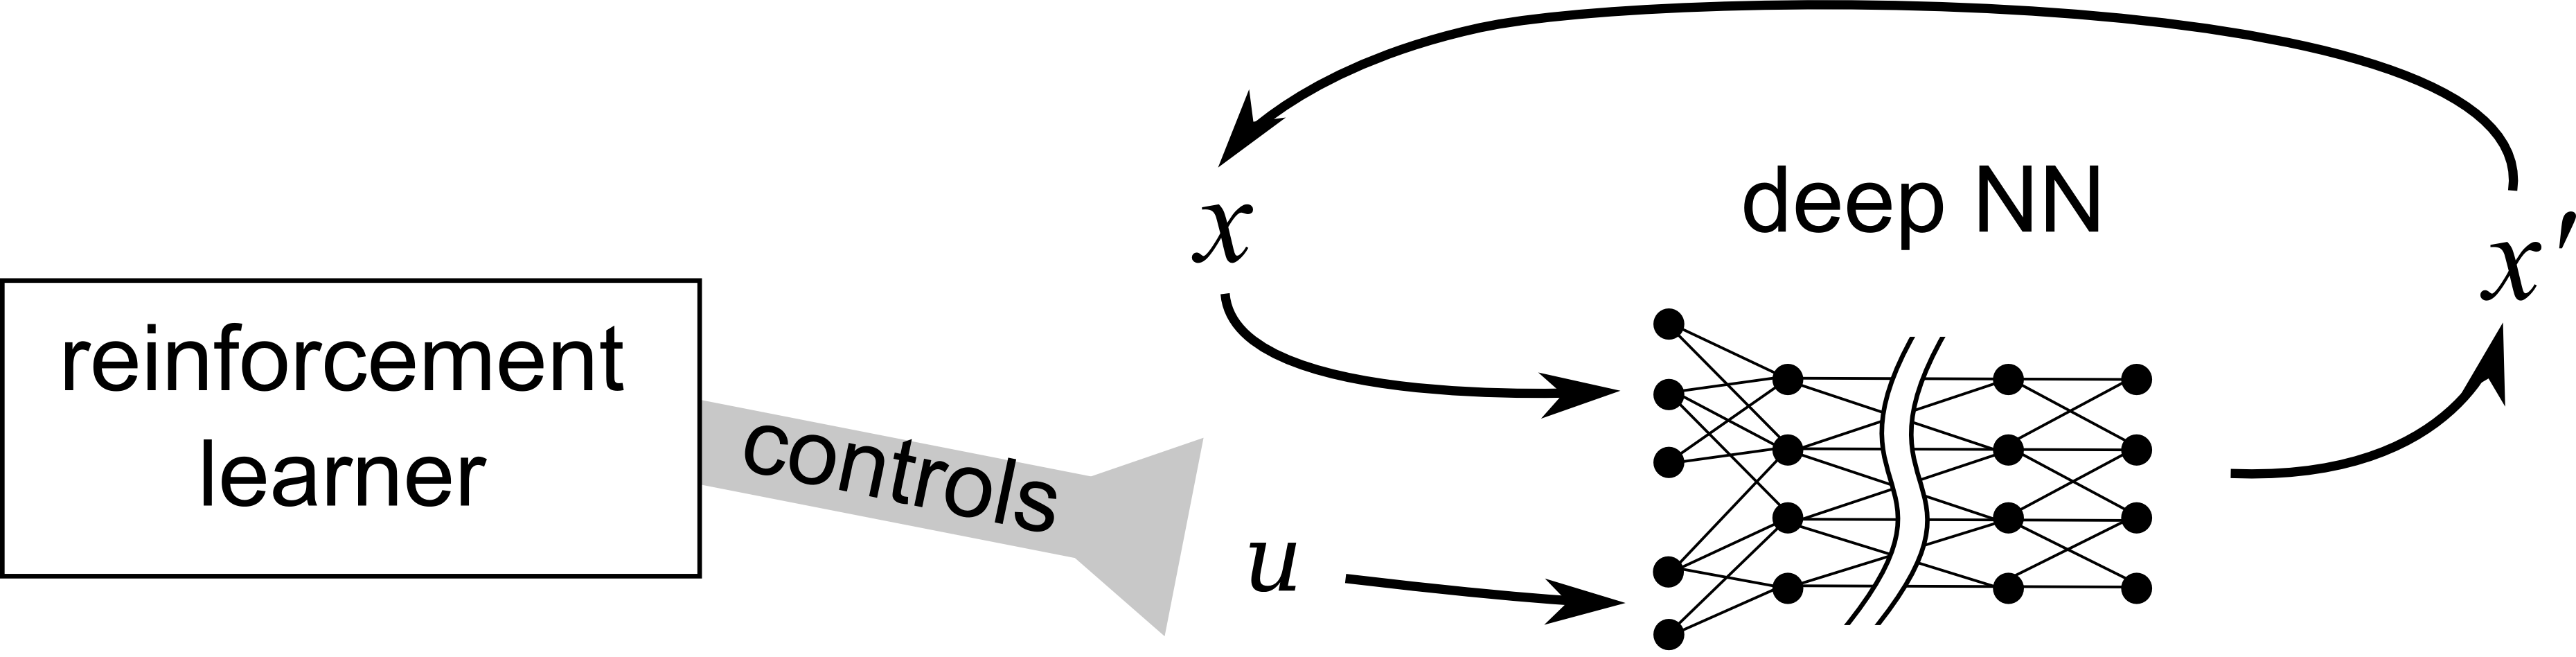
\includegraphics[scale=0.5]{model-with-u.png}
\end{equation}
But such a neural network requires a novel learning algorithm that is \textbf{reward-driven} rather than the traditionally \textbf{error-driven} back-propagation.  Such an algorithm is difficult to design because it cannot rely on old-fashioned gradient descent.

One solution that avoids the difficulty is to make the neural network compute the Q-value:
\begin{equation}
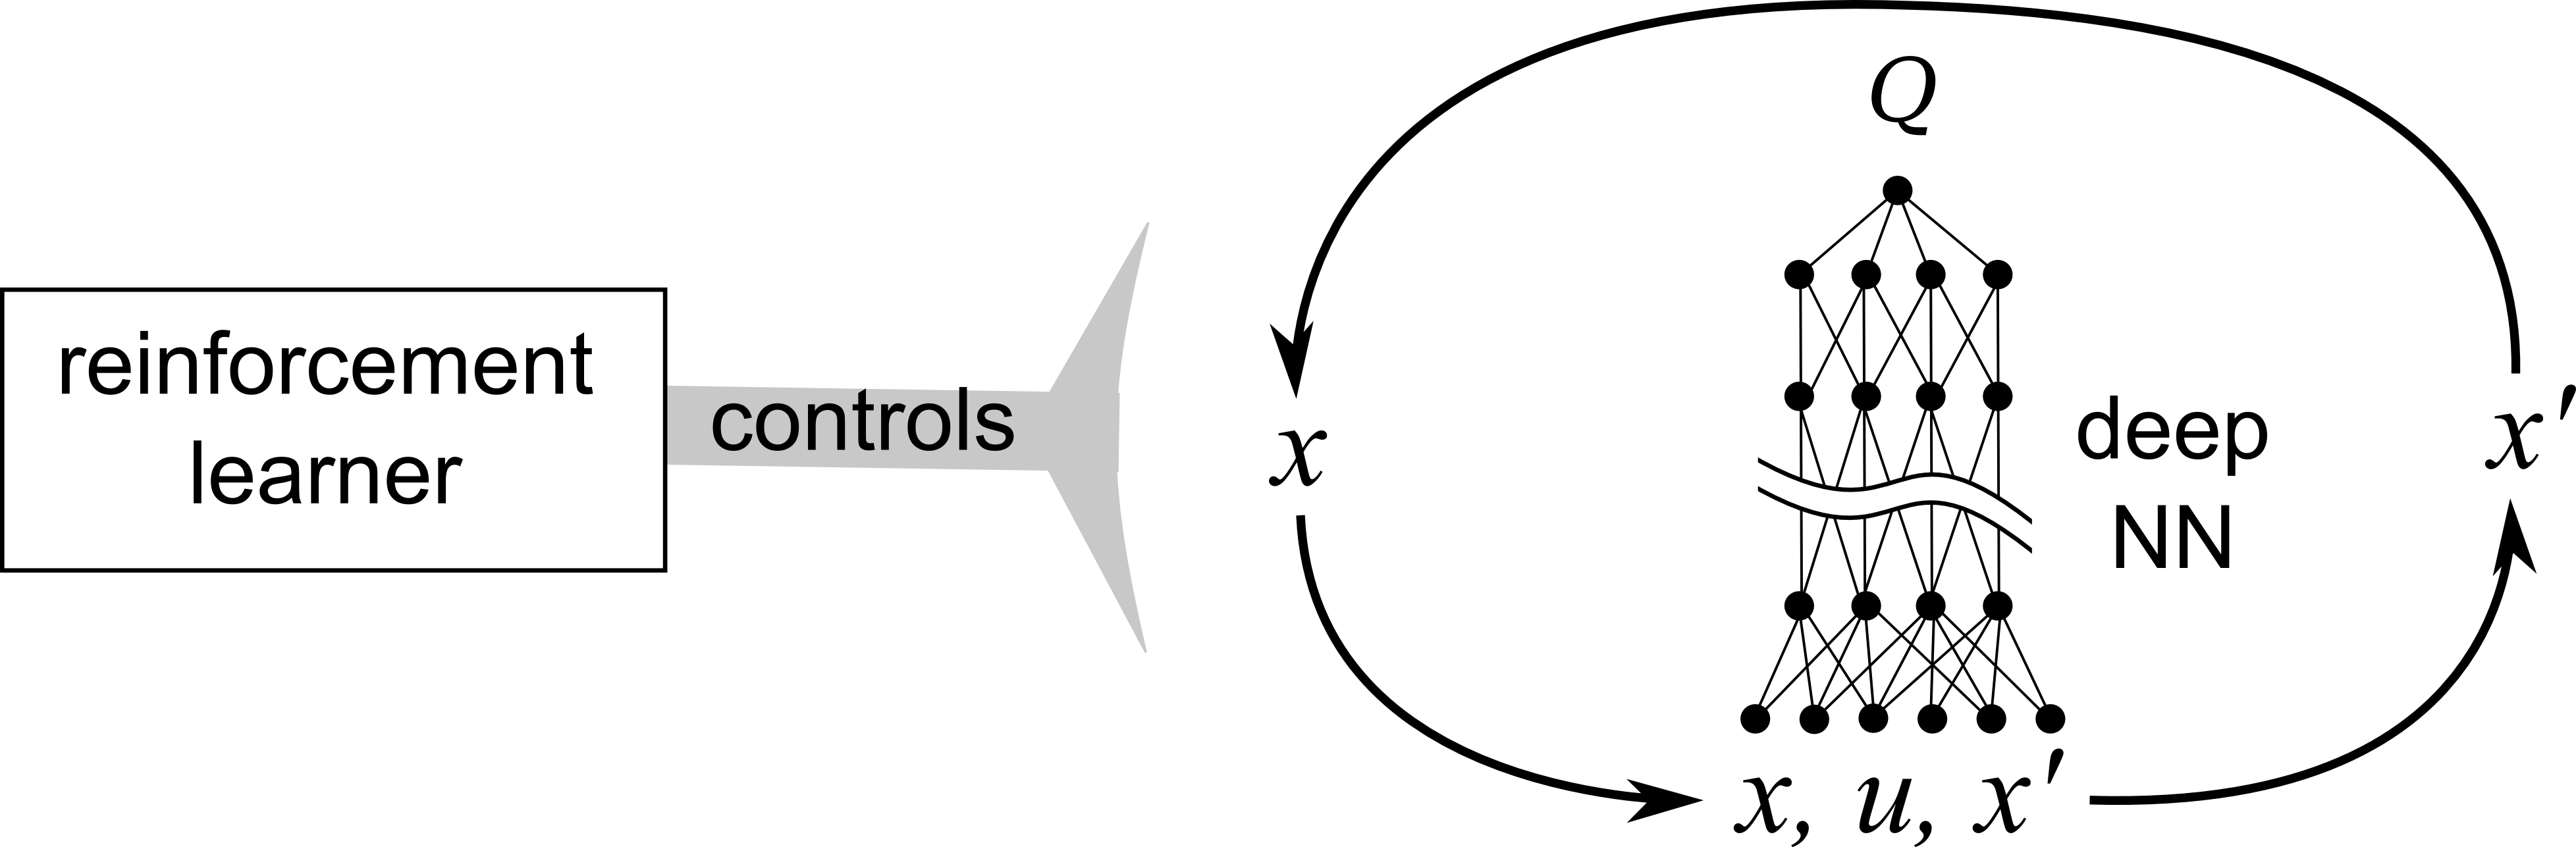
\includegraphics[scale=0.5]{model-Sayaka.png}
\end{equation}
This means that we can compute $Q$ for any transition $x \stackrel{u}{\mapsto} x'$.  During the ``action'' (ie, ``thinking'') stage, we hold $x$ fixed, and search for $(u, x')$ that maximizes $Q$;  This can be done by \textbf{stochastic gradient descent}.  During the ``learning'' stage, we are given certain transitions $(x, u, x')$ and we train the neural network to adjust $Q$ via standard \textbf{Bellman update}.

% ================================== comment out ==================================
\iffalse

From the viewpoint of reinforcement learning, we aim to learn the \emp{policy} function: \par
\begin{equation}
\begin{tikzcd}[]
\mbox{policy : ~~state} \arrow[r, mapsto, "\scalebox{0.8}{action}"] & \mbox{state'}
\end{tikzcd}
\end{equation}
Where $K$ can be regarded as the \emp{mental state}, and thus an \emp{action} in RL turns $K$ into $K'$.

In our system, there are 2 pathways that act on $K$, via RNN and RL respectively: \par
\begin{equation}
\begin{tikzcd}[column sep=huge]
& K'_1 \arrow[dd, dashed, no head, "\scalebox{1.3}{$\approx$}"] \\
K \arrow[ur, "\mbox{RL}"] \arrow[dr, "\mbox{RNN}"'] & \\
& K'_2
\end{tikzcd}
\end{equation}
In RL, the action $a$ acts on $K$, whereas in RNN, $R$ acts on $K$.

\emp{Note}: RNN and RL are learning algorithms, and if they are both applied to the same problem, conflicts will necessarily arise, unless there is a way to combine them.

At state $K$, we estimate the Q-value $Q(K \stackrel{a}{\mapsto} K')$.  The action that would be chosen at state $K$ is $\displaystyle \arg\max_a Q(K \stackrel{a}{\mapsto} K')$.  This could be used to train the RNN via $\displaystyle K \vdash_W ...^n K'$.

RL 在众多状态 $K$ 之间游荡,学习 $Q(K \mapsto K')$。  因为 RL 独有奖励讯息,我们必需用 RL 来教导 RNN 学习,反之不可。  第一个问题是: RL 如何在 $K$ 之间游荡?   游荡是随机的,但也可以借助 RNN 的随机性、或在 RNN 自身的游荡中注入更多随机性、或者根本就是 RL 自己产生的随机性。  接下来的问题是: RNN 如何用 $Q$ 值来诱发学习?

RNN 的 ``$n$-fold'' 学习可以通过以下方式实现: 
\begin{itemize}
\item stochastic forward-backward propagation
\item genetic?
\item 最有趣的是 Hebbian learning,因为它似乎特别适合这情况。  
\end{itemize}

RNN 的本质是什么?  它似乎是一个 recurrent hetero-associative memory。  但其实它还需要将 input 作类似於 Word2vec 的 encoding。  这个 encoding 将「相似」的思维状态 $K$ 归到同类。  利用空间中的相似度,RL 可以用一些连续函数来近似 Q 值(详细情况还有待分析)。

另一个问题是: 虽然用函数的近似可以做到 generalization,但另一个方法是利用状态 $K$ 中的空位作暂时储存。 这两者似乎很不同。  问题似乎在於: 状态转换 $K \mapsto K'$ 是不是对应於逻辑中的\emp{一条} rule?  答案似乎是 yes。  这个共识是很重要的。  如果用 decision tree,需要的是向量空间中的相似度。

现在的关键是「状态变量」。  因为它可以做到符号逻辑中靠变量的 generalization,这是前所未有的。  这种 generalization 似乎不需要相似度,因为它是符号的!  会不会在向量空间中的状态变量 能够做到之前逻辑变量做不到的动作?  不管怎样,用 RNN 学习这些变量的动作似乎是很难的,因为这些动作似乎不是对\emp{误差}的梯度下降。  除非这些动作本身也近似於其他动作,但那是怎样的近似?  学习 multi-step logic 其实和以前的 forward / backward chaining 没有分别!  唯一分别是命题的 representation 改变了,它未必像符号的 concatenation。  所以问题仍然是 ``$n$-fold'' 学习法。 

而且注意: RL 的 generalization 根本上不同於 rules 空间中的 generalization。 前者是思维空间 $K$ 中的一般化,后者也可以是 $K$ 空间的一般化,但也可以是依赖「状态变量」的一般化。

一般来说,RL 和 RNN 的行动和学习,是可以互相独立的。  

还有 heterarchical 的分类法。  想用 decision tree 或什么,达到不同网络的\emp{分工}。  在组织知识这方面,深度网络有没有用?  可以想像,在视觉识别中,在网络的最上层有很多 objects,而它们都可以还原到底层的 features。  网络有更多层,可以识别的事物更抽象。  但现在我们要的不是\emp{模式识别},而是 mapping。 特别是抽象模式的 mapping。  想要的是: 大量的 rules,将不同的 $K$ 映射到新的 $K'$。

还有一点要澄清的是: 究竟每一个「思元素」在向量空间中是不是\emp{一点}?  如果有了这个「思元素 = 点」假设,则每次 iteration 应该会删除一个思元素,而用另一个(全新的)思元素取代之。  这样,$K \mapsto K'$ mapping 就有了更确定的结构。  这样的 setup 已经很接近 logic 系统,但其学习算法仍然很有 combinatorial 的 ``feel''。 (因为只有当两个 rules 串连之后,才能达到某个结论,而这个串连有没有中间的 continuous 状态?)  这种串连通常是怎样找到的?  

现在有一转机: 如果「思元素 = 点」,则「状态变量」的形成似乎会很普遍,而我们可以集中研究如何学习 single-step rules。 RL 的 rewards 可以指导学习,但这些「终极 rewards」对学习的细节没有指导作用。  我们似乎可以用「\emp{时间延迟}」来达到「状态变量」的效果,这个做法无形中增加了使用状态变量的机会。  

现在总结一下仍然有待回答的问题:
\begin{itemize}
\item RL 的 generalization 如何做?
\item iterative thinking map 如何 learn?
\item 
\end{itemize}

Hebbian 的情况是: 有某一 I/O pattern; 我想 strengthen 这 pattern。 

Assuming the learning is correct, $K'_1$ and $K'_2$ should be roughly the same \textemdash~ but this ignored the possibility that one path may take multiple steps to converge with the other path.  \footnote{This situation has been encountered in term rewriting systems (TRS):  If in a TRS any 2 different rewriting paths always converge to the same result, it is said to have the \emp{Church-Rosser property}.  For example the $\lambda$-calculus invented by Church has this property.} 

Now I stipulate that $R$ be more ``refined'', that is to say, applying $D^n$ times may be equivalent to applying $a$ once:
\begin{equation}
\begin{tikzcd}[column sep=huge]
& K'_1 \arrow[dd, dashed, no head, "\scalebox{1.3}{$\approx$}"] \\
K \arrow[ur, "\scalebox{1.3}{$a$}"] \arrow[dr, "{\scalebox{1.3}{$D^n$}}"'] & \\
& K'_2
\end{tikzcd}
\end{equation}
Using a different notation, $a$ is the \emp{restriction} or \emp{section} of $D^n$ at point $K$: $a = D^n|_K$.

Now the question is, do the RNN and RL paths have any \textit{essential} difference?
\begin{itemize}
\item Their internal \emp{representations} are different:\par
\dashh RNN is a multi-layer neural network\par
\dashh RL's representation is $Q(\mbox{state},\mbox{action})$, usually stored as a \textit{look-up table}, although $Q$ could be approximated by a neural network as well.
\item RL learns through \emp{rewards}, RNN learns from \emp{errors}.  Thus RL has broader applicability, because not all questions have ``correct answers'' that could be measured by errors.  In RL we just need to praise Genifer whenever she displays good behavior.
\item The internal cognitive state $K$ exists because of RNN:  it is simply the vector input and output of the RNN.  Without this $K$, RL would be clueless as to what are its internal states.  It can be said that the RNN provides a \textit{machinery} for RL to control.
\end{itemize}

% programming needed:
% RNN: with special back-prop
% RL: approximate Q(K,a), using special NN that can find max also

% 整体来说,RL 可以操控的 actions 包括:
% \begin{enumerate}[\tab (A)]
% \item apply $K \stackrel{D}{\mapsto} K'$ \par
% 但注意: $K$ 是认知状态,$R$ 是对 $K$ 进行「合乎逻辑的推论」。 所以,无论发生什么事,我们都会将 $R$ 作用在 $K$ 上几次。 换句话说,$R$ 是\ds{必然}进行的动作,或者可以看成是在\ds{背景}下进行的运作,所以不需要用 RL 学习。 %RL 的用处是学习如何在很多 actions 之间选择最好的一个,所以 $R$ 不是 RL 需要学习的 action,它只是。

% \item 改写认知状态 $K \mapsto K'$ \par
% RL 的 actions (A) 是
% 在思考过程中改变 $K$ 的值。 例如我们得到一个局部结论,这个局部结论的状态不是最终答案,但也比什么都没有的效用更高。 改写 $K$ 的方法可以是: 例如 将 $K \mbox{ += } \delta K$,或者 「if $K \in$ 某 region,then $K \mbox{ += } \delta K $」。

% \item 学习: change $R$ \par

From the perspective of reinforcement learning, we could reward some results of multi-step inference: \par
\begin{equation}
\begin{tikzcd}[row sep=tiny]
K_0 \arrow[r, mapsto, "\scalebox{1.3}{$a$}"] & K_\vdash \quad \updownarrow \bigstar
\end{tikzcd}
\end{equation}
$\updownarrow \bigstar$ means ``to give positive or negative rewards''.  We want to learn $a$ which is the action to be taken at state $K$.  The learning algorithm is based on the famous \emp{Bellman optimality condition} (see next section).

Perhaps we should use RL to \textit{guide} the learning in RNN, as RNN is more fine-grained....

To combine the 2 learning approaches, we could use the technique of \emp{interleaving}: for each step apply RL once, apply RNN $n$ times.

% 但 $R$ 本身是 RNN,它还可以透过 back-prop 进行学习,两者似乎是不同的。  Back-prop 是透过 $\frac{\partial}{\partial D}(\mbox{error})$ 的梯度来学习。

The learning in RNN may also involve \emp{neurogenesis} (adding new neurons and connections), but I have not considered this aspect yet.

% RNN 的 $R$ 也是将 $K$ 变成 $K'$ 的作用:\par
%\begin{figure}[h]
%\centering
%\begin{tikzcd}[row sep=tiny]
%K \arrow[r, mapsto, "\scalebox{1.3}{$R$}"] & K'
%\end{tikzcd}
%\end{figure}
% $R$ 和 RL 的 actions 是不一样的。

There are 4 learning modes:
\begin{itemize}
\item learning to listen/talk
\item RL-based learning
\item inductive learning
\end{itemize}

\section{Misc points}

\begin{itemize}
\item If sigmoid is replaced by polynomial, universal approximating property may be retained.

\item Banach fixed point theorem does not apply because $R$ in general need not be contractive.  Question is whether $R$ necessarily converges to fixed points and the answer is no.

\item If reasoning operator $R$ is continuous, the flow of the dynamical system is governed by an autonomous differential equation.  Poincare-Bendixson only applies to dynamical systems on the plane, and is irrelevant to systems whose phase space has dimension $\geq 3$, or to discrete dynamical systems.

\item Time can be discrete or continuous.

\item Goal is to find minimizer of error (ie, to approximate a function given some input-output data points).  The (finite) set of local minima can be solved via setting $\frac{\partial R}{\partial W} = 0$.  The number of local minima can be calculated as: ?  McClelland paper.

\item If operator is discontinuous, what advantages can be gained?
\end{itemize}

What I want to do now is to determine if $R$ implemented as a deep network is sufficient to model human-level reasoning.

One principle seems to be that logical conclusions must not proliferate indefinitely.  But we are not sure what kind of structural constraints this would impose on the vector space.  Or whether we should impose such constraints manually.

What other properties are desired for the implementation of $R$?

\section{Architecture}

First, cartoon version:
\begin{equation}
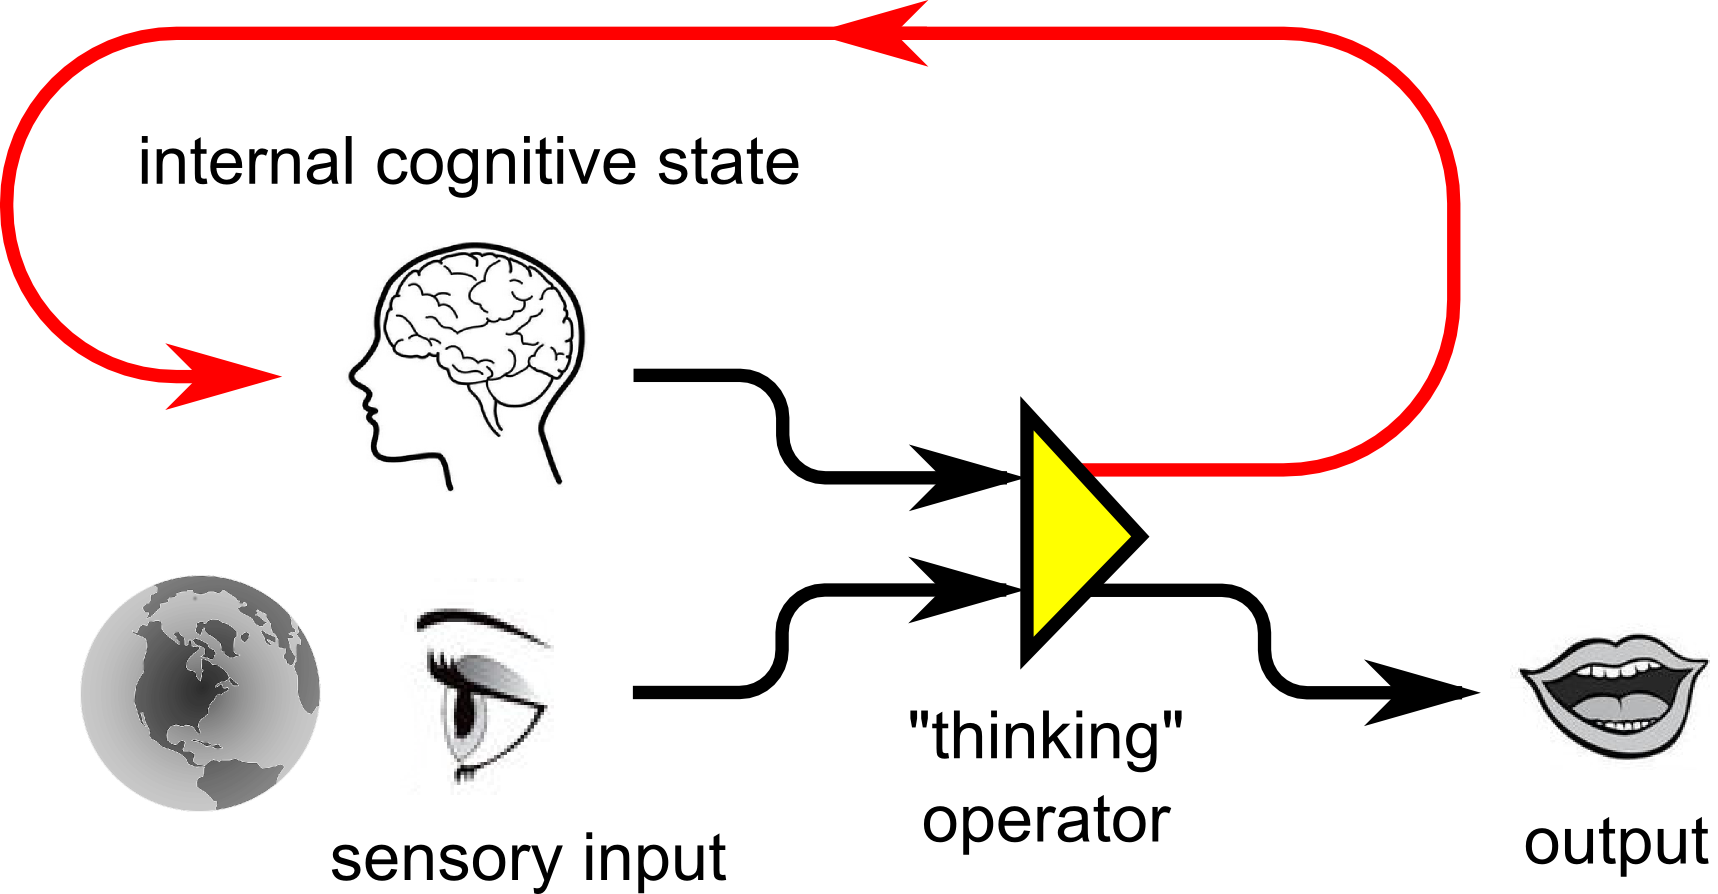
\includegraphics[scale=0.5]{architecture-cartoon.png}
\end{equation}

\begin{equation}
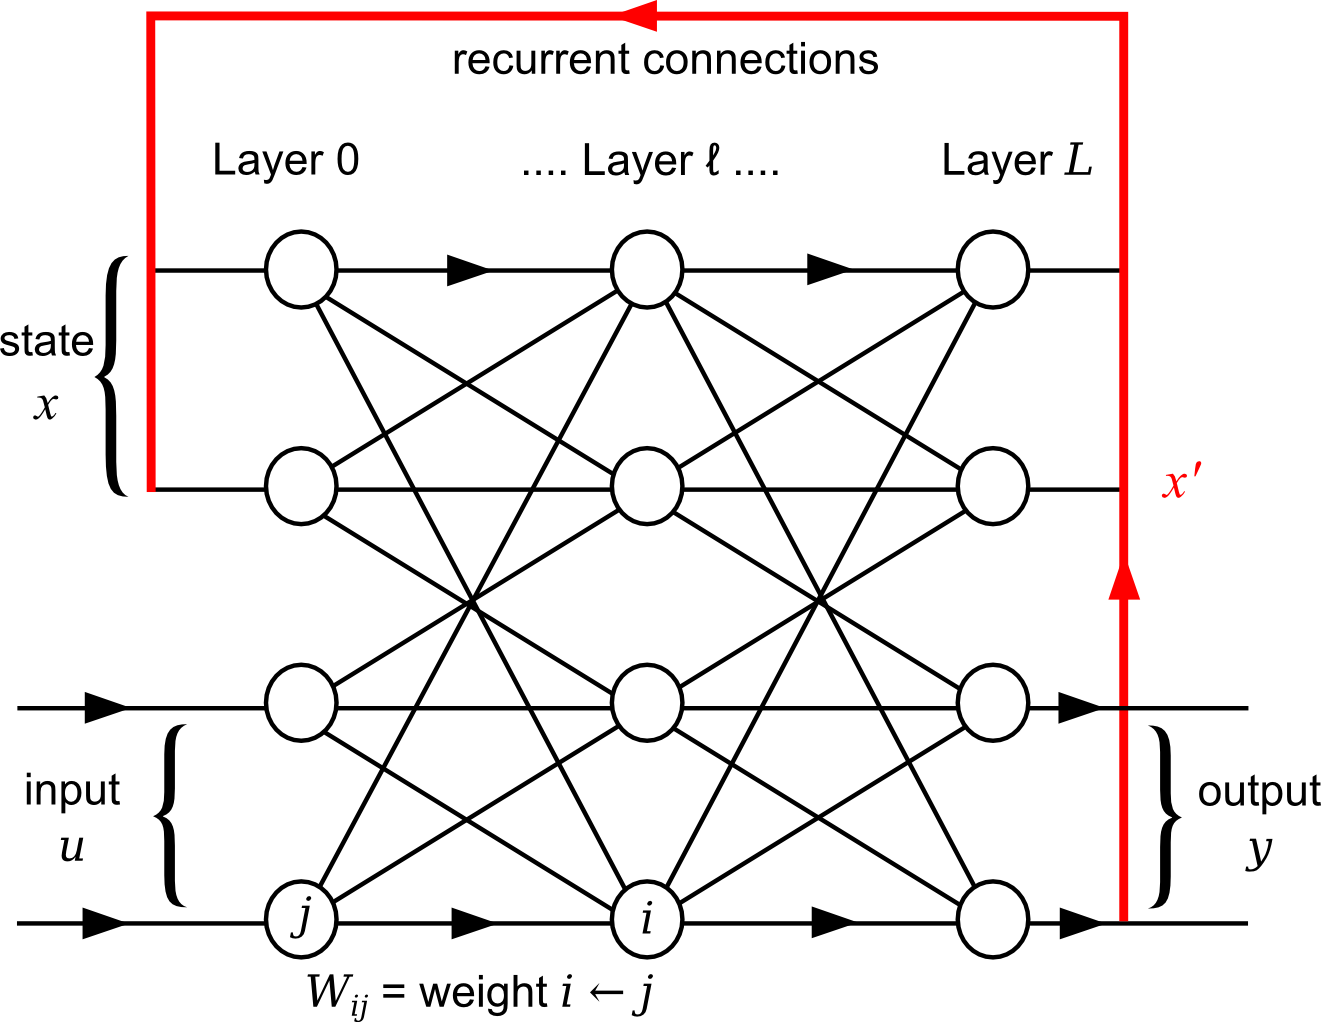
\includegraphics[scale=0.5]{RNN-topology.png}
\end{equation}

TO-DO:  The state space $X$ may be too large and we may need an \emp{attention mechanism} to select some parts of $X$ for processing by $R$.  This is the notion of \emp{working memory} in cognitive science.
\begin{equation}
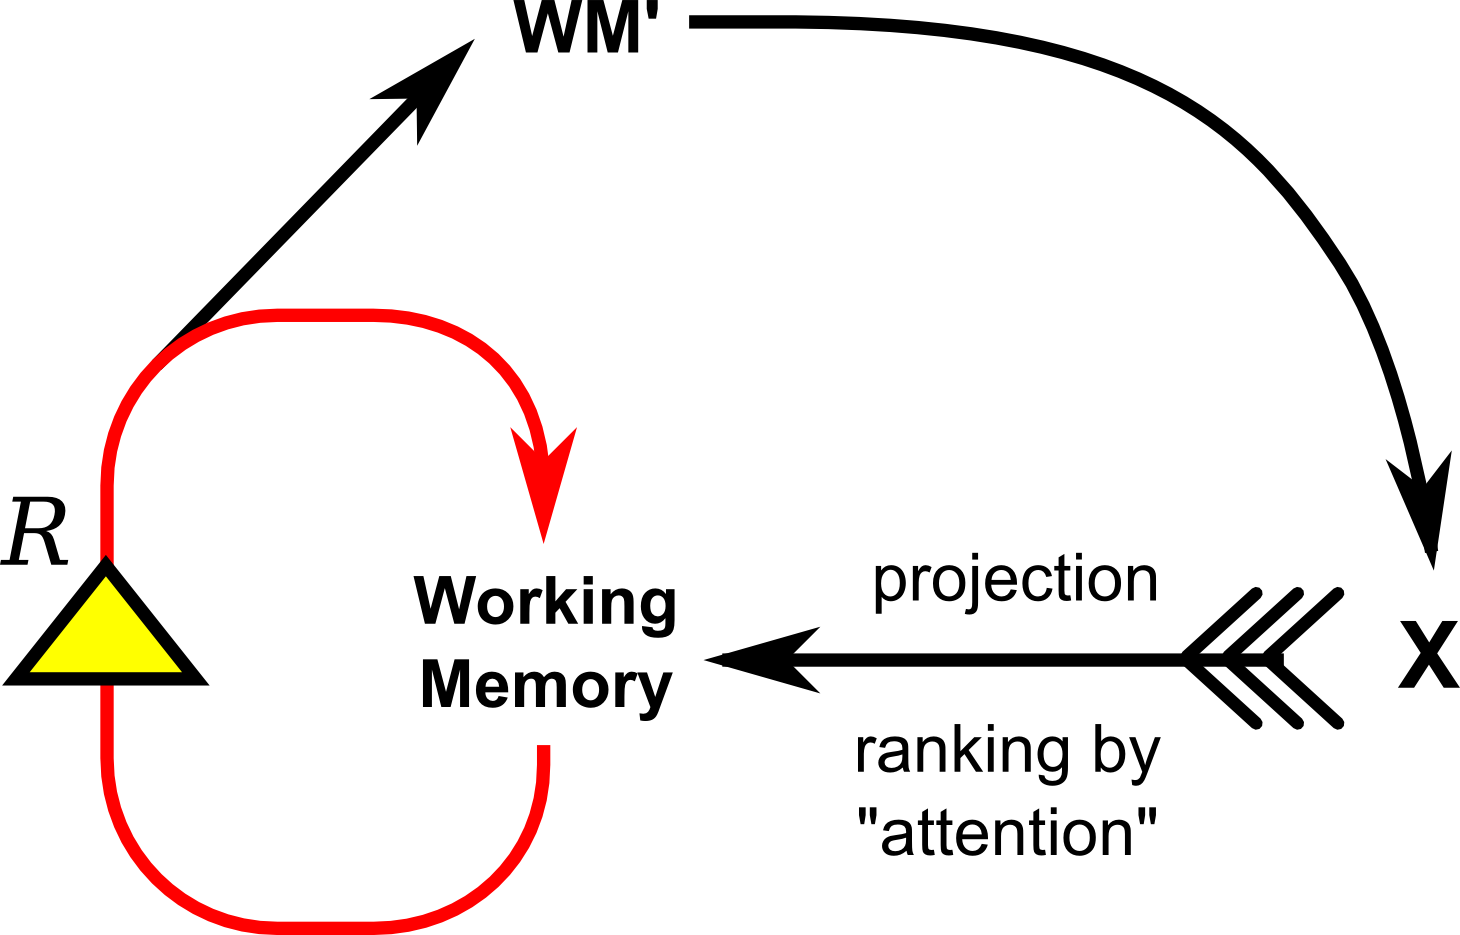
\includegraphics[scale=0.4]{working-memory.png}
\end{equation}

\section{Deep Recurrent Learning}

The learning algorithm for $R$ is central to our system.  $R$ learns to recognize input-output pairs $( \vec{x}_0, \vec{x}^* )$.  What makes it special is that $R$ is allowed to iterate a \textit{flexible} number of times before outputting an answer.  In feed-forward learning we simply learn single-pass recognition, whereas in common recurrent learning we train against a \textit{fixed} time sequence.  Here, the time delay between input and output is allowed to stretch arbitrarily.

Suppose the recurrent network $R$ iterates $n$ times:
\begin{equation}
\vec{x}_{t+1} = \overbrace{R \circ R \circ ...}^{n} (\vec{x})
\end{equation}

As $n \rightarrow \infty$, we get the continuous-time version (a differential equation):
\begin{equation}
\frac{d\vec{x}(t)}{dt} = \mathfrak{R}(\vec{x}(t))
\end{equation}

We could run the network $R$ for a long enough time $T$ such that it is highly likely to reach an equilibrium point.  Then:
\begin{equation}
\vec{x}_{T} = \int_0^T \mathfrak{R}(\vec{x}(t)) dt
\end{equation}
and the error:
\begin{equation}
\mathscr{E} = \vec{x}^* - \vec{x}_{T}
\end{equation}
where $\vec{x}^*$ is the target value which is independent of time.
\begin{eqnarray}
\frac{\partial\mathscr{E}}{\partial\vec{W}} &=& - \frac{\partial}{\partial\vec{W}} \int_0^T \mathfrak{R}(\vec{x}(t)) dt \nonumber \\
&=& - \frac{\partial}{\partial\vec{W}} \int_0^T \sigmoid(W_1 \sigmoid(W_2 ... \sigmoid(W_L \vec{x}(t))) dt
\end{eqnarray}

When there are many layers or if the recurrence is too long, back-prop learning becomes ineffective due to the \emp{vanishing gradient} problem.  One solution is to use the \emp{rectifier} activation function:
\begin{equation}
\rectifier (x) = 
\begin{cases}
x, & \mbox{if } x \geq 0 \\
0, & \mbox{otherwise}
\end{cases}
\end{equation}
Since its derivative is piecewise constant, it does not suffer from the vanishing gradient problem.

\subsection{Forward-backward Algorithm}

This is inspired by forward- and backward-chaining in LBAI.  We propagate the state vector from both the initial state $\vec{x}_0$ as well as the final state $\vec{x}^*$.  This bi-directional propagation is added with noise and repeated many times, thus implementing a \emp{stochastic local search}:

\begin{equation}
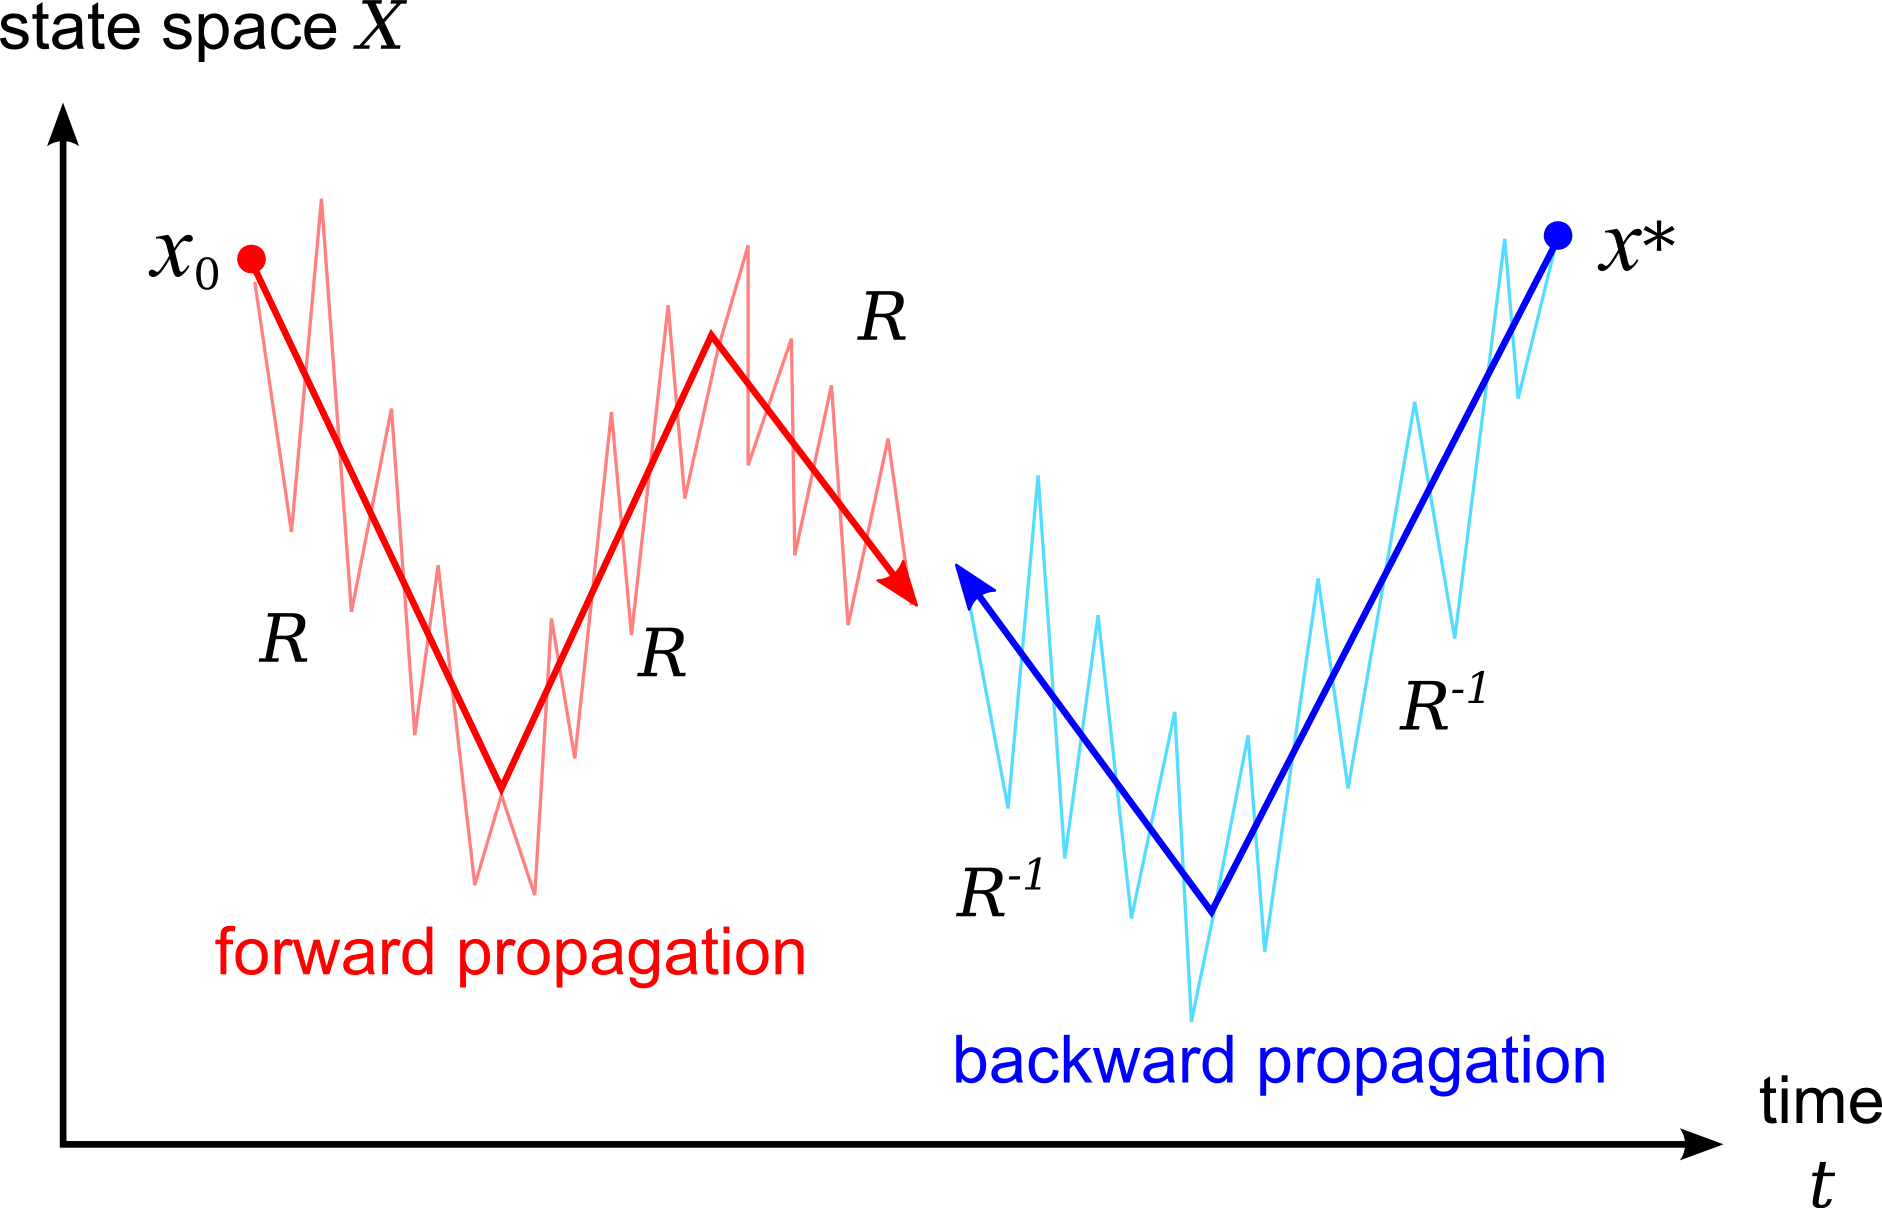
\includegraphics[scale=0.6]{forward-backward-algorithm.png}
\end{equation}

When the forward and backward states get close enough, a successful path is found, and we record the gap and the noises along the path, and use them to train $R$ so that this new path would be recognized.

% One key question is how to deal with "don't care" bits?  One answer is that their errors are zero.  But then this is the same as the error for "correct" weights, which seems not well.  There's got to be a way to alter weights when the answer is correct...

% For \# Iteration = 0, output is immediately known, so potentially the training can be done.  But how to convey that all these alterations of weights are \emp{optional}?

% \section{Reinforcement learning}

% ================================== comment out ==================================
\fi

\section*{Acknowledgement}

\footnotesize{In a forum discussion with Ben Goertzel dated 25 June 2014 on the AGI mailing-list: (agi@listbox.com), YKY asked: Why bother with neural networks, which typically require many neurons to encode data, when logic-based AI can represent a proposition with just a few symbols?  Ben's insight is that neural networks are capable of learning their own representations, and their learning algorithms are relatively speaking much faster.  We have been working on "neo-classical" logic-based AI for a long time, and began to realize that inductive learning in logic (based on combinatorial search in a symbolic space) is perhaps \textit{the bottleneck} in the entire logic-based paradigm.  So we try to look for alternatives that might learn faster, though we would still emphasize that logic-based AI remains a viable approach to AGI. %, provided that the right search heuristics be found (most probably in the form of \emp{hierarchical organization} of the learning space).
}

\bibliographystyle{plain} % or number or aaai ...
\bibliography{AGI-book}

\end{document}
